\documentclass[12pt]{article}

\usepackage[spanish]{babel}
\usepackage[utf8]{inputenc}
\usepackage[T1]{fontenc}
\usepackage{graphicx}
\usepackage{amsmath}
\usepackage{booktabs}
\usepackage{geometry}
\usepackage{float}
\usepackage{hyperref}
\usepackage{xcolor}
\usepackage{listings}

% Configuración para que el código Python se vea bonito
\definecolor{codegreen}{rgb}{0,0.6,0}
\definecolor{codegray}{rgb}{0.5,0.5,0.5}
\definecolor{codepurple}{rgb}{0.58,0,0.82}
\definecolor{backcolour}{rgb}{0.95,0.95,0.92}

\lstdefinestyle{estiloPython}{
    backgroundcolor=\color{backcolour},   
    commentstyle=\color{codegreen},
    keywordstyle=\color{blue},
    numberstyle=\tiny\color{codegray},
    stringstyle=\color{codepurple},
    basicstyle=\ttfamily\footnotesize,
    breakatwhitespace=false,         
    breaklines=true,                 
    captionpos=b,                    
    keepspaces=true,                 
    numbers=left,                    
    numbersep=5pt,                  
    showspaces=false,                
    showstringspaces=false,
    showtabs=false,                  
    tabsize=4,
    language=Python
}
\lstset{style=estiloPython}

\geometry{margin=2.5cm}

\begin{document}

\begin{titlepage}
\begin{center}

% Si tienes el logo en la misma carpeta, déjalo así. Si no, ajusta la ruta.

\includegraphics[width=5cm]{logo_ugr.png}

\vspace{1cm}

{\Huge \textbf{Metaheurísticas}}

\vspace{0.5cm}

{\Large Práctica 1 \\
    Planificación de Exámenes Universitarios mediante Búsqueda Local}

\vspace{1.5cm}

\textbf{Ilias Ahmed Ahmed}

\vfill

22--03--2026

\end{center}
\end{titlepage}

% Índice en su propia página
\newpage
\tableofcontents
\newpage

\section{Introducción}
En esta práctica he abordado el problema propuesto en la práctica de la planificación de exámenes universitarios. Este tipo de problemas se caracteriza por tener un espacio de búsqueda exponencial, lo que hace inviable encontrar la solución más óptima con métodos exactos en un tiempo computacional razonable a medida que crece el tamaño de la instancia.

El objetivo principal consiste en asignar un conjunto de exámenes a diferentes franjas horarias (slots) y aulas, garantizando el cumplimiento de una serie de restricciones obligatorias (duras) y minimizando al mismo tiempo ciertas penalizaciones (restricciones blandas) que reflejan la calidad final que tendra el horario generado para los estudiantes.

Para resolver este desafío, he utilizado técnicas heurísticas de búsqueda local como se indica en el enunciado. Partiendo de una solución inicial construida de forma aleatoria, el algoritmo explora iterativamente el vecindario de la solución actual realizando pequeños movimientos. En concreto, he implementado y comparado las dos estrategias principales que hemos estudiado:
\begin{itemize}
    \item \textbf{Búsqueda de primer mejor:} Acepta el primer vecino generado que mejore el valor de la función objetivo con respecto a la solución inicial.
    \item \textbf{Búsqueda del mejor vecino:} Evalúa un subconjunto del vecindario y selecciona el que proporcione la mayor mejora.
\end{itemize}

Todo el desarrollo, incluyendo la generación de instancias, evaluación, cambios en el vecindario y generación de gráficas, se ha realizado íntegramente en Python utilizando librerías estándar como \texttt{numpy}, \texttt{pandas} y \texttt{matplotlib}.

\section{Modelado del problema}
\subsection{Representación de la solución}
He decidido representar cada posible solución (estado) mediante un diccionario (tabla hash) en Python, donde la clave es el identificador del examen y el valor es una tupla que contiene la franja horaria y el aula asignada:
\texttt{examen -> (slot, aula)}

He tomado esta decisión de diseño por tres motivos principales:
\begin{itemize}
    \item \textbf{Eficiencia de acceso:} Permite consultar la asignación de cualquier examen en tiempo constante $O(1)$.
    \item \textbf{Facilidad de cambio:} En los algoritmos de búsqueda local, la operación más frecuente es la modificación de la solución. Un diccionario permite actualizar asignaciones de forma inmediata, directa y sencilla.
    \item \textbf{Garantiza unicidad:} Al ser el examen la clave del diccionario, la propia estructura de datos garantiza que un examen no pueda ser asignado a más de un slot o aula simultáneamente (cumpliendo automáticamente la tercera restricción dura del enunciado).
\end{itemize}

\subsection{Restricciones del problema}
El problema exige el cumplimiento de tres restricciones duras:
\begin{itemize}
    \item \textbf{No solapamiento por estudiante:} Un estudiante no puede examinarse de dos asignaturas simultáneamente. Para verificar esto de forma eficiente, he precalculado un diccionario \texttt{mapa\_estudiantes} (estudiante -> lista de exámenes). Así, al evaluar, solo recorro los exámenes de cada estudiante y compruebo mediante un \texttt{set} si hay slots duplicados.
    \item \textbf{Capacidad del aula:} El número de matriculados en un examen debe ser menor o igual al aforo del aula asignada.
    \item \textbf{Asignación única:} Como mencioné en el apartado anterior, la propia estructura de datos elegida garantiza que cada examen se programe exactamente una vez.
\end{itemize}

\subsection{Tratamiento de las restricciones en la búsqueda}
He decidido adoptar un enfoque de penalización de restricciones duras. En lugar de obligar al algoritmo a visitar únicamente soluciones factibles (lo cual limitaría enormemente la conectividad del espacio de búsqueda y haría muy complejo diseñar operadores de vecindario), permito que el algoritmo transite por soluciones inválidas.

Para que esto funcione, he introducido una fuerte penalización en la función objetivo. Las ventajas de esta decisión son:
\begin{itemize}
    \item Evita que la búsqueda local se quede estancada muy rápido en óptimos locales por culpa de "muros" de casos no factibles.
    \item Simplifica enormemente la lógica de los operadores de mutación, ya que no tienen que validar que la mutación es factible tras cada cambio.
\end{itemize}

\section{Función objetivo}
Para evaluar la calidad de un horario, he diseñado una función objetivo que transforma el problema en un modelo de minimización de costes. La formulación matemática que he implementado es la siguiente: 

$$f(x) = W_1 \cdot P_{consecutivos} + W_2 \cdot P_{mismo\_dia} + W_3 \cdot P_{distribucion} + W_v \cdot V$$

Donde los pesos asignados y justificados son:
\begin{itemize}
    \item $P_{consecutivos}$ ($W_1 = 1$): Penaliza si un estudiante tiene exámenes en slots seguidos ($slot_i$ y $slot_{i+1}$). Se calcula ordenando los slots de cada estudiante. Le he asignado el peso base de 1.
    \item $P_{mismo\_dia}$ ($W_2 = 2$): Penaliza tener múltiples exámenes en la misma jornada (asumiendo jornadas de 5 slots). Le he dado un peso el doble de estricto que los consecutivos, ya que a nivel de fatiga y saturación mental para un alumno, hacer dos o tres exámenes en un mismo día es un defecto grave de planificación.
    \item $P_{distribucion}$ ($W_3 = 1$): He utilizado la varianza del uso de los slots. Una varianza cercana a 0 indica que los exámenes están perfectamente repartidos a lo largo de todas las franjas horarias.
    \item Restricciones duras ($W_v = 100000$): He asignado un peso desproporcionadamente alto (100000) a cada incumplimiento de restricción dura (solapamiento o exceso de aforo). De esta forma, cualquier solución factible siempre será matemáticamente superior a una infactible.
\end{itemize}

\section{Generación de instancias}
Para la experimentación, he diseñado un generador de instancias utilizando \texttt{numpy} y \texttt{pandas}. He fijado la semilla aleatoria (\texttt{seed=42}) para aislar el comportamiento estocástico/aleatorio y garantizar que mis algoritmos sean reproducibles cada vez que los ejecuto.

Las dimensiones de la instancia base que he utilizado en estos resultados son:
\begin{itemize}
    \item 100 exámenes
    \item 2000 estudiantes (cada uno matriculado en un número aleatorio de entre 3 y 6 asignaturas).
    \item 10 aulas (con capacidades aleatorias entre 30 y 200).
    \item 40 franjas horarias (slots).
\end{itemize}

Para garantizar que los algoritmos se prueban en un entorno realista y heterogéneo, el generador de instancias distribuye a los alumnos de forma desigual. Como se puede observar en el siguiente histograma (correspondiente a la instancia Media), la gran mayoría de exámenes concentran a un número moderado de estudiantes, mientras que unos pocos exámenes actúan como eventos multitudinarios, lo que añade una capa de dificultad real al problema de asignación de aulas.

\begin{figure}[H]
    \centering
    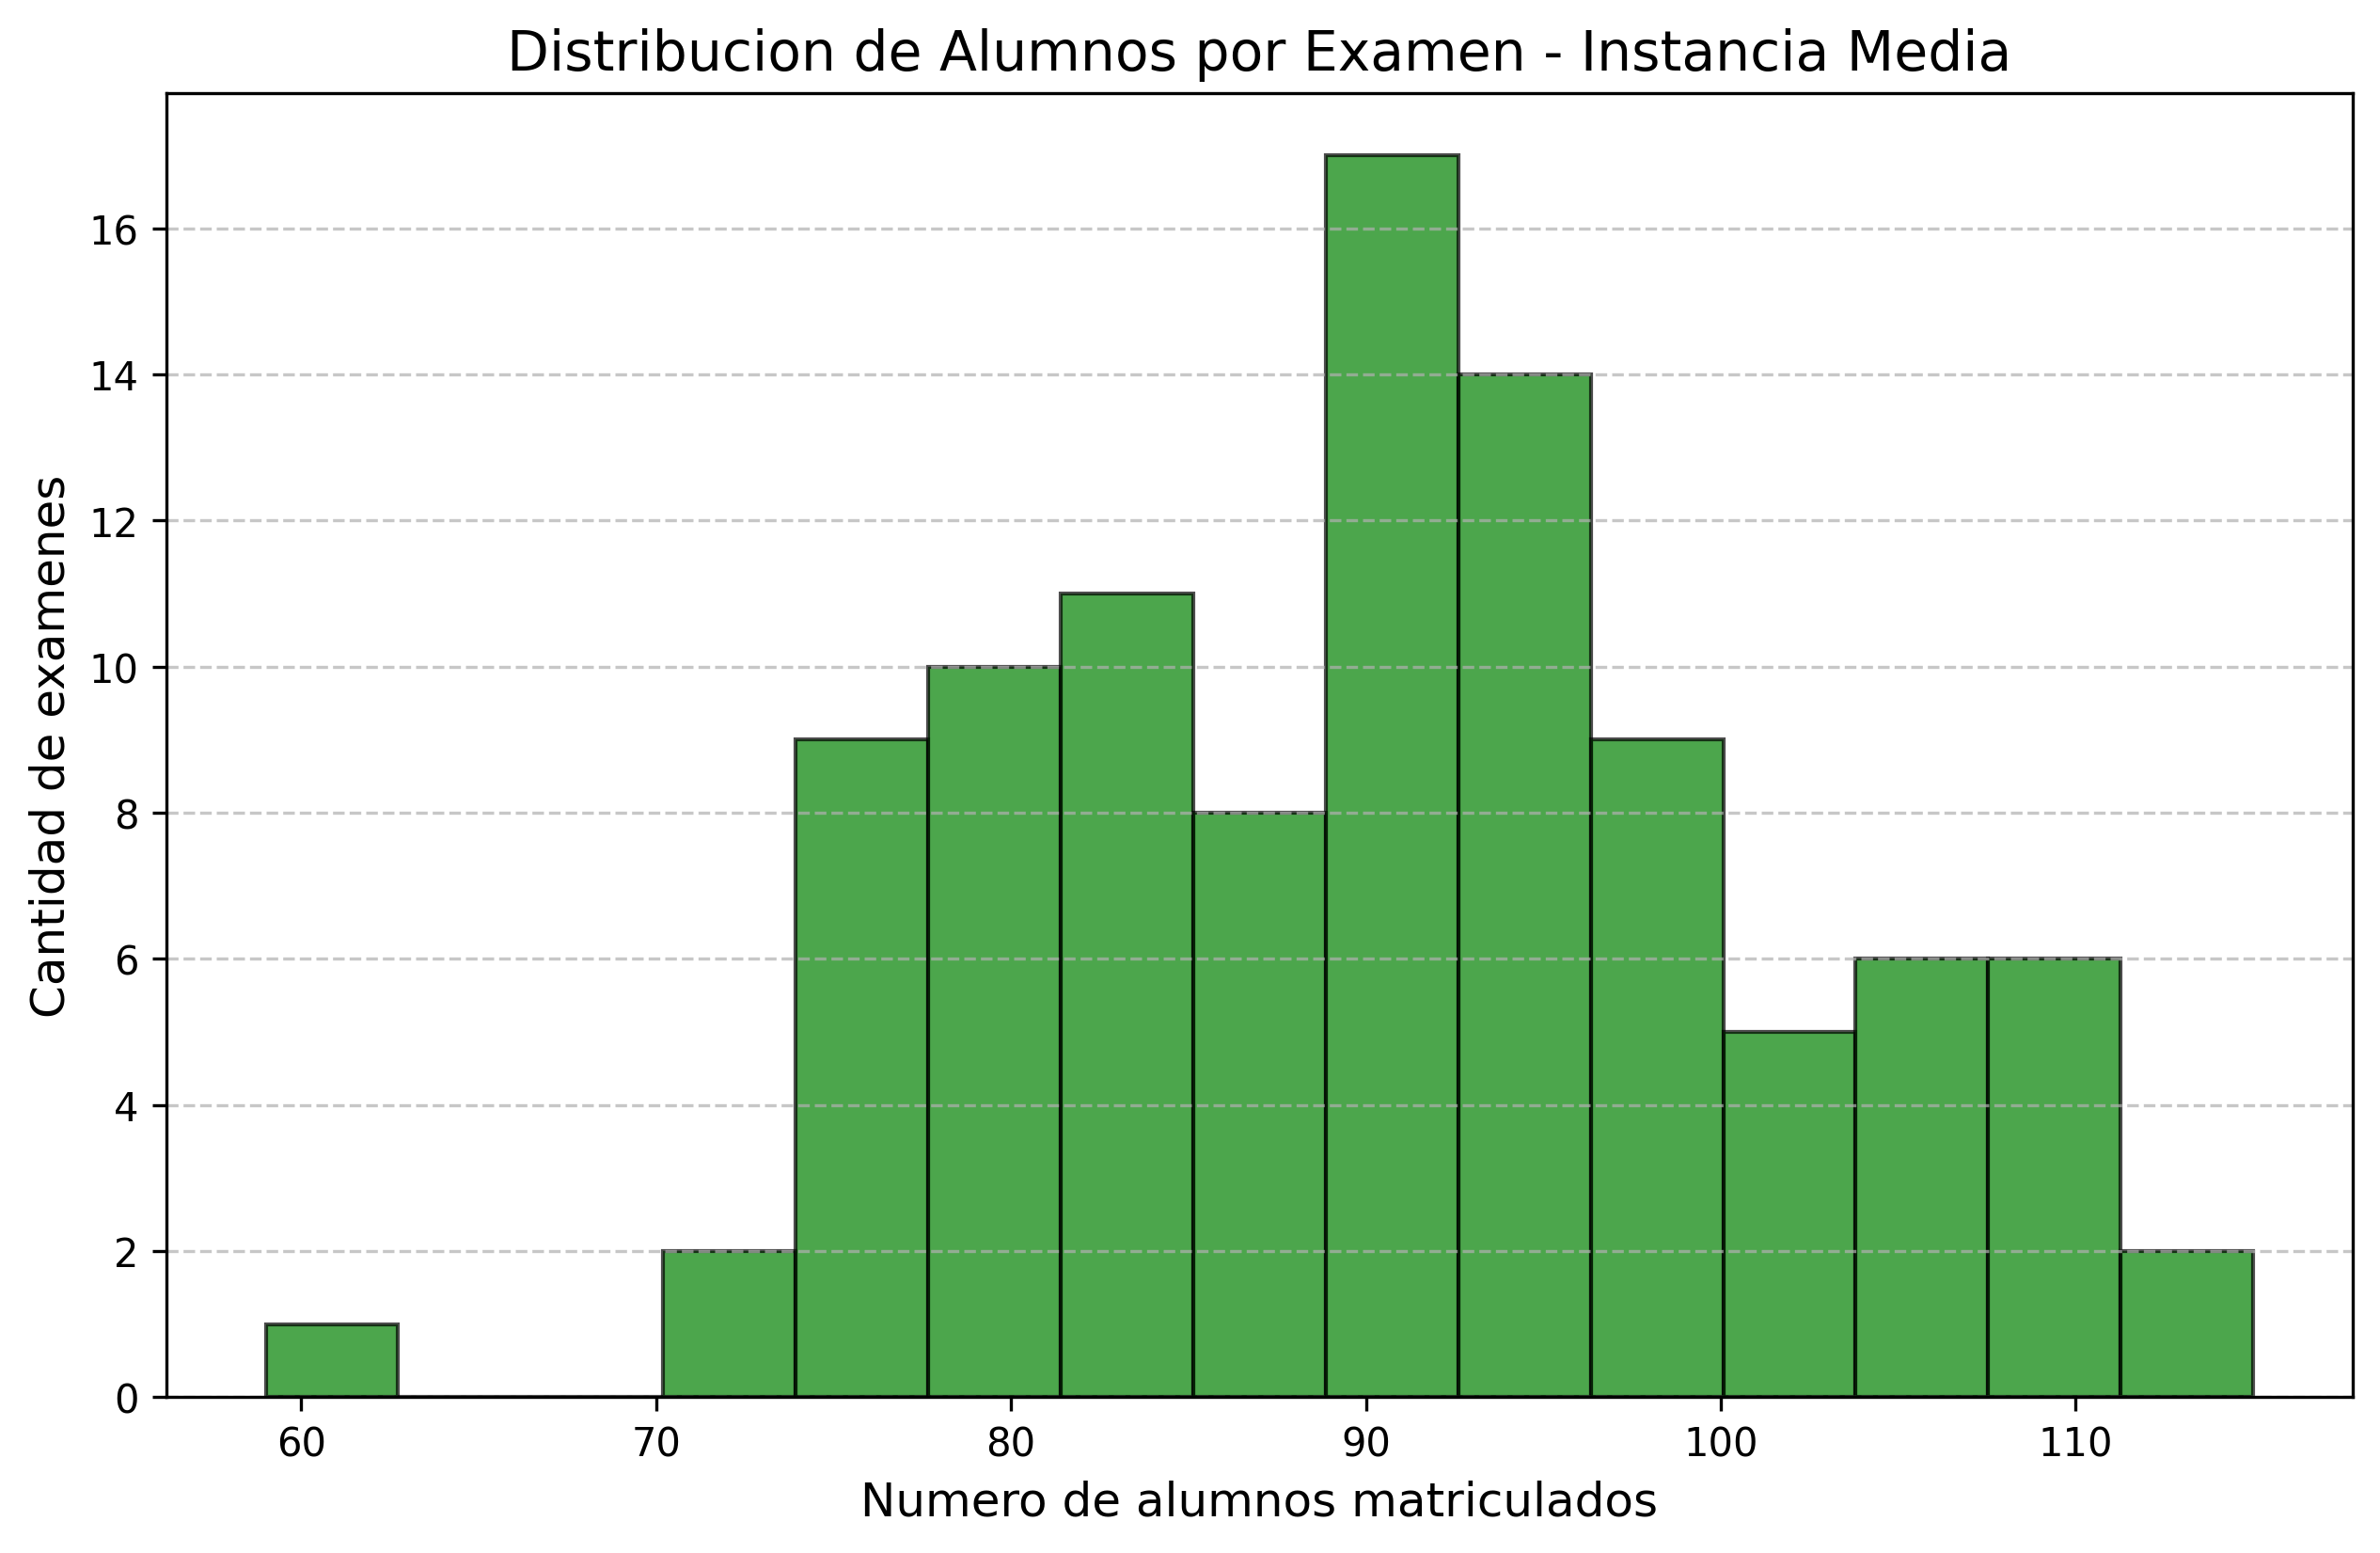
\includegraphics[width=0.8\textwidth]{graficas/histograma_alumnos.png}
    \caption{Distribución de alumnos matriculados por examen.}
\end{figure}

\section{Solución inicial}
La construcción de la solución inicial (\texttt{solucion\_inicial}) la he realizado mediante una heurística aleatoria. Para cada examen, el algoritmo genera aleatoriamente un slot y un aula, e intenta validar únicamente que la capacidad sea suficiente (con un límite de 100 intentos). Si no encuentra hueco, lo asigna a la fuerza.

Esta estrategia me genera un punto de partida de muy baja calidad (con numerosos conflictos y incumplimientos), pero tiene la gran ventaja de ser computacionalmente instantánea (0.01 segundos), pasando todo el esfuerzo de optimización a la metaheurística que se encarga del resto del proceso.

\section{Vecindario}
El operador de vecindario es el motor de la búsqueda local, lo que hace que vaya pasando de un vecino a otro y evaluandolos entre sí. He diseñado un generador aleatorio (\texttt{generar\_vecino}) que cambia la solución actual aplicando uno de estos tres movimientos de forma aleatoria:
\begin{itemize}
    \item \textbf{Cambio de slot:} Selecciona un examen al azar y le reasigna una franja horaria completamente aleatoria.
    \item \textbf{Cambio de aula:} Selecciona un examen al azar y le reasigna un aula diferente.
    \item \textbf{Intercambio (Swap):} Selecciona dos exámenes aleatorios e intercambia entre sí sus configuraciones completas (slot y aula).
\end{itemize}

He combinado estos movimientos de un solo componente (cambios de slot o aula) con movimientos de dos componentes (swaps). Los primeros permiten hacer pequeños ajustes que son menos sensibles, mientras que los swaps permiten realizar saltos un poco más grandes en el espacio de búsqueda, lo que es fundamental para intentar escapar de óptimos locales y no quedarse atascado pero sin destrozar completamente la estructura de la solución que estábamos evaluando.

\section{Búsqueda local}
He implementado las dos variantes que se nos pedían, añadiendo un criterio de parada híbrido para evitar ejecuciones infinitas: la búsqueda se detiene si se alcanza el máximo de iteraciones globales (\texttt{max\_iter=5000}) o si en una iteración completa no se encuentra ninguna mejora que sería un estancamiento en óptimo local.

\subsection{Estrategia de Primer Mejor}
En cada iteración de la búsqueda, el algoritmo explora el vecindario generando vecinos de forma aleatoria pero de manera controlada dentro de las 3 opciones que comenté anteriormente. Evalúa uno a uno y, en el momento en que encuentra uno cuyo coste es menor que el actual, acepta el movimiento de forma inmediata y avanza al siguiente estado.

\subsection{Estrategia de Mejor Vecino}
A diferencia del anterior, este método genera una muestra representativa del vecindario (he fijado un límite exploratorio de 500 vecinos aleatorios por iteración debido a que el tamaño total del vecindario es enorme). Evalúa los 500 vecinos sin realizar ningún movimiento, y solo al final de la exploración adopta el mejor de ellos, siempre y cuando mejore el coste actual.

\section{Implementación y estructura del código}
Para mantener el proyecto organizado y no volverme loco buscando errores en un único archivo gigante, decidí aplicar una arquitectura modular. He separado la lógica en distintos archivos \texttt{.py} según su función que desempeñan. De esta forma, el código es mucho más limpio, tiene sentido lógico y es más fácil de mantener.

A continuación, explico cómo he planteado cada módulo desde mi punto de vista y qué hace exactamente:

\subsection{\texttt{generaInstancias.py}}
Para este módulo, he partido del código base que se nos proporcionaba en el enunciado de la práctica. En vez de dejar ese código suelto al principio de mi programa principal, decidí encapsularlo todo dentro de una única función \texttt{generar\_instancia()}.

Lo que hace es usar \texttt{numpy} y \texttt{pandas} para inventarse los estudiantes, los exámenes y las capacidades de las aulas. Al meterlo en una función, me aseguro de que me devuelva exactamente las cuatro variables limpias que necesito (\texttt{student\_exam}, \texttt{exams}, \texttt{rooms}, \texttt{n\_slots}). Además, le he dejado la semilla aleatoria fija (\texttt{seed=42}). Esto es crucial para mí, porque si la instancia cambiaba en cada ejecución, me resultaba imposible saber si mis algoritmos estaban mejorando o si simplemente les había tocado un escenario con otros datos más fácil.

\subsection{\texttt{inicial.py}}
Este archivo es el paso previo antes de empezar a usar la metaheurística. Lo dividí en dos funciones para hacerlo más sencillo:

\textbf{\texttt{construir\_mapa\_estudiantes()}:} Durante el desarrollo, me topé con un problema de rendimiento gravísimo. La estructura de datos original generada era un DataFrame de Pandas larguísimo con miles de filas emparejando [Estudiante, Examen]. El problema es que, en cada una de las miles de evaluaciones que hace la búsqueda local, el algoritmo necesita comprobar si algún alumno tiene exámenes solapados. 

Para solucionarlo, creé esta función. Lo que hace es recorrer la tabla una sola vez antes de empezar a optimizar, y lo agrupa todo en un diccionario nativo de Python (el mapa). En este diccionario, la clave es el estudiante y el valor es su lista de exámenes (ejemplo: \texttt{alumno\_54 : [Examen\_2, Examen\_14]}). Gracias a este pre-cálculo, consultar los exámenes de cualquier alumno durante la búsqueda pasa a ser de acceso directo e instantáneo en memoria ($O(1)$). Lo que antes ahogaba a la CPU, ahora se ejecuta en milisegundos.

\textbf{\texttt{solucion\_inicial()}:} Aquí genero el primer horario (el que luego vamos a optimizar). Mi estrategia fue simple: asigno slots y aulas al azar, comprobando únicamente que el aforo de la clase sea suficiente (con un tope de 100 intentos para no quedarme en un bucle infinito). No me preocupo si a un alumno le coinciden dos exámenes; prefiero generar una solución rápida aunque sea mala, y dejar que la búsqueda local se encargue de arreglar la posible mala primera solución después.

\subsection{\texttt{funcionObjetivo.py}}
Este archivo es el núcleo matemático del proyecto. En lugar de hacer una función muy larga y compleja, programé pequeñas funciones independientes para cada problema: una para contar exámenes en días seguidos (\texttt{penalizacion\_consecutivos}), otra para exámenes en el mismo día (\texttt{penalizacion\_mismo\_dia}), otra para ver qué tan bien repartidos están (\texttt{penalizacion\_distribucion}), y la más importante, la que cuenta los solapamientos y excesos de aforo (restricciones duras).

Finalmente, la función principal \texttt{evaluar\_detallado()} las llama a todas y suma los puntos multiplicando por los pesos que definí en la teoría. Aquí es donde puse el multiplicador bestial de $100000 \cdot v$ a los incumplimientos de restricciones para que el algoritmo huya de los horarios ilegales.

\begin{lstlisting}[caption={Función de evaluación detallada en Python}]
def evaluar_detallado(sol, exams, rooms, mapa_estudiantes, n_slots):
    p1 = penalizacion_consecutivos(sol, mapa_estudiantes)
    p2 = penalizacion_mismo_dia(sol, mapa_estudiantes)
    p3 = penalizacion_distribucion(sol, n_slots)
    v = incumplimientos(sol, exams, rooms, mapa_estudiantes)
    total = p1 + 2*p2 + p3 + 100000*v
    return total, p1, p2, p3, v
\end{lstlisting}

\subsection{\texttt{busquedaLocal.py}}
Aquí es donde realmente ocurre lo principal de la práctica. Contiene los dos algoritmos que se nos pedían (\texttt{busqueda\_primer\_mejor} y \texttt{busqueda\_mejor}). Para no repetir código en ambos, me creé una función auxiliar llamada \texttt{generar\_vecino()}.

\texttt{generar\_vecino()}: Es la encargada de hacer las "mutaciones". Tira una especie de dado de tres caras (\texttt{random.randint(0, 2)}): si sale 0, cambia la hora de un examen; si sale 1, le cambia el aula; y si sale 2, intercambia por completo dos exámenes de sitio (swap). Los algoritmos en sí son bucles \texttt{while} que no paran hasta que llegan al máximo de evaluaciones (\texttt{max\_iter=5000}) o hasta que se dan cuenta de que ningún vecino nuevo mejora lo que ya tienen (momento en el que se rinden por estancamiento).

\subsection{\texttt{main.py}}
Este script actúa como el "director de orquesta" de toda la práctica. Es el punto de entrada del programa y se encarga de coordinar e importar los diferentes módulos que se han descrito anteriormente para automatizar la batería de pruebas de principio a fin.

El núcleo del archivo es la función \texttt{ejecutar\_experimentos()}, donde se han definido directamente los parámetros de los tres escenarios de escalabilidad (instancias Pequeña, Media y Grande). Mediante un bucle iterativo, el script recorre cada uno de estos escenarios y ejecuta el flujo completo de resolución:
\begin{enumerate}
    \item Genera la instancia concreta apoyándose en el módulo de generación.
    \item Construye la estructura auxiliar (mapa de estudiantes) y la solución inicial aleatoria.
    \item Lanza la optimización utilizando la estrategia de Primer Mejor y cronometra su ejecución usando la librería estándar \texttt{time}.
    \item Repite el proceso de optimización, partiendo de la misma solución inicial, pero aplicando la estrategia de Mejor Vecino, cronometrando también su tiempo.
\end{enumerate}

Además de orquestar el flujo lógico, este archivo cumple una doble función vital en la recolección y presentación de resultados:
\begin{itemize}
    \item \textbf{Salida por consola:} Imprime un registro detallado de las evaluaciones, penalizaciones y incumplimientos de restricciones duras de cada algoritmo paso a paso, culminando en la impresión de una tabla resumen perfectamente tabulada con los costes y tiempos comparados.
    \item \textbf{Integración visual:} Recopila durante el bucle todos los arrays de evolución de costes y las métricas finales para, justo antes de terminar la ejecución, llamar a las funciones del módulo \texttt{graficas.py}. De esta forma, automatiza la creación y guardado de todas las figuras analíticas utilizadas en los apartados posteriores de esta memoria.
\end{itemize}

\subsection{Módulo de visualización de resultados (\texttt{graficas.py})}
Para facilitar el análisis de los datos y automatizar la creación de las figuras incluidas en esta memoria, se ha implementado un módulo específico apoyado en las librerías \texttt{matplotlib} y \texttt{numpy}.

La principal ventaja de extraer esta lógica a un archivo independiente es mantener el script principal (\texttt{main.py}) limpio y enfocado exclusivamente en la ejecución de las metaheurísticas. Al inicio de este archivo, se utiliza la librería \texttt{os} para crear automáticamente una carpeta llamada \texttt{graficas} en el directorio del proyecto, asegurando que todas las imágenes generadas se guarden allí sin ensuciar el espacio de trabajo.

El módulo cuenta con tres funciones principales, cada una destinada a un tipo de análisis visual diferente:
\begin{itemize}
    \item \textbf{\texttt{grafica\_convergencia()}:} Recibe los arrays con el historial de costes devueltos por los algoritmos y genera un gráfico de líneas. Es fundamental para observar el descenso del coste iteración a iteración y comprobar visualmente en qué punto exacto cada algoritmo se estanca o colapsa.
    \item \textbf{\texttt{graficas\_comparativas()}:} Toma las listas con los resultados finales (costes y tiempos) de todos los tamaños de instancia y genera dos gráficos de barras agrupadas. Permite comparar de un solo vistazo el rendimiento del "Primer Mejor" frente al "Mejor Vecino" a medida que el problema sufre la explosión combinatoria.
    \item \textbf{\texttt{histograma\_alumnos()}:} Recibe el listado de exámenes de una instancia y genera un histograma de frecuencias. Su propósito es validar que el generador de instancias funciona correctamente, demostrando que la distribución de alumnos es heterogénea y realista (con unas pocas asignaturas muy pobladas y muchas asignaturas con pocos alumnos).
\end{itemize}

\subsection{Dificultades encontradas y soluciones}
Quería mencionar también un par de problemas que me fueron surgiendo durante el desarrollo del código y cómo los solucioné:
\begin{itemize}
    \item \textbf{El cuello de botella de la evaluación:} Como comenté en el apartado del \texttt{inicial.py}, al principio mi programa recorría las tablas de pandas constantemente. Esto hacía que la búsqueda local fuera demasiado lenta cada vez que quería ejecutar el programa. La solución de crear el diccionario \texttt{mapa\_estudiantes} me ahorró mucho tiempo de ejecución a lo largo de todo el proyecto, reduciendo el tiempo de evaluación drásticamente y logrando hacer miles de iteraciones en apenas unos segundos.
    \item \textbf{El problema de las referencias al generar vecinos:} Cuando empecé a programar la función \texttt{generar\_vecino()}, me volví loco porque al probar un cambio en el horario para ver si era mejor, ¡también se me estaba modificando la solución actual sin querer! Esto pasaba porque en Python los diccionarios se pasan por referencia. Me costó un rato ver el fallo, pero lo solucioné creando una copia auxiliar al inicio del generador (\texttt{nuevo = dict(sol)}) para poder hacer pruebas con el vecino sin destrozar la solución original.
\end{itemize}

\section{Resultados obtenidos}
Al ejecutar \texttt{main.py} llamando a todos los módulos y poniendo a competir a ambos algoritmos con la misma instancia inicial, he obtenido los siguientes datos empíricos:

\begin{table}[H]
\centering
\begin{tabular}{lrrr}
\toprule
\textbf{Métrica} & \textbf{Solución Inicial} & \textbf{Primer Mejor} & \textbf{Mejor Vecino} \\
\midrule
Coste Total & 33,704,554.6 & 8,704,058.3 & 22,704,264.95 \\
Incumplimientos (Duras) & 337 & 87 & 227 \\
Penalización Consecutivos & 833 & 792 & 788 \\
Penalización Mismo Día & 1860 & 1633 & 1738 \\
Tiempo de Ejecución & 0.0107 s & 43.42 s & 48.33 s \\
Evaluaciones Totales & N/A & 4702 & 5000 \\
Iteraciones (Mejoras) & N/A & 139 & 10 \\
\bottomrule
\end{tabular}
\caption{Comparativa de métricas en la Instancia Media (100 exámenes).}
\end{table}

Aunque no se haya llegado a 0 incumplimientos de las restricciones duras debido a la altísima densidad de la instancia (100 exámenes y 2000 estudiantes para solo 10 aulas) y al número máximo de evaluaciones impuesto, se puede observar una reducción drástica respecto al inicio, demostrando que la heurística funciona.

\begin{figure}[H]
    \centering
    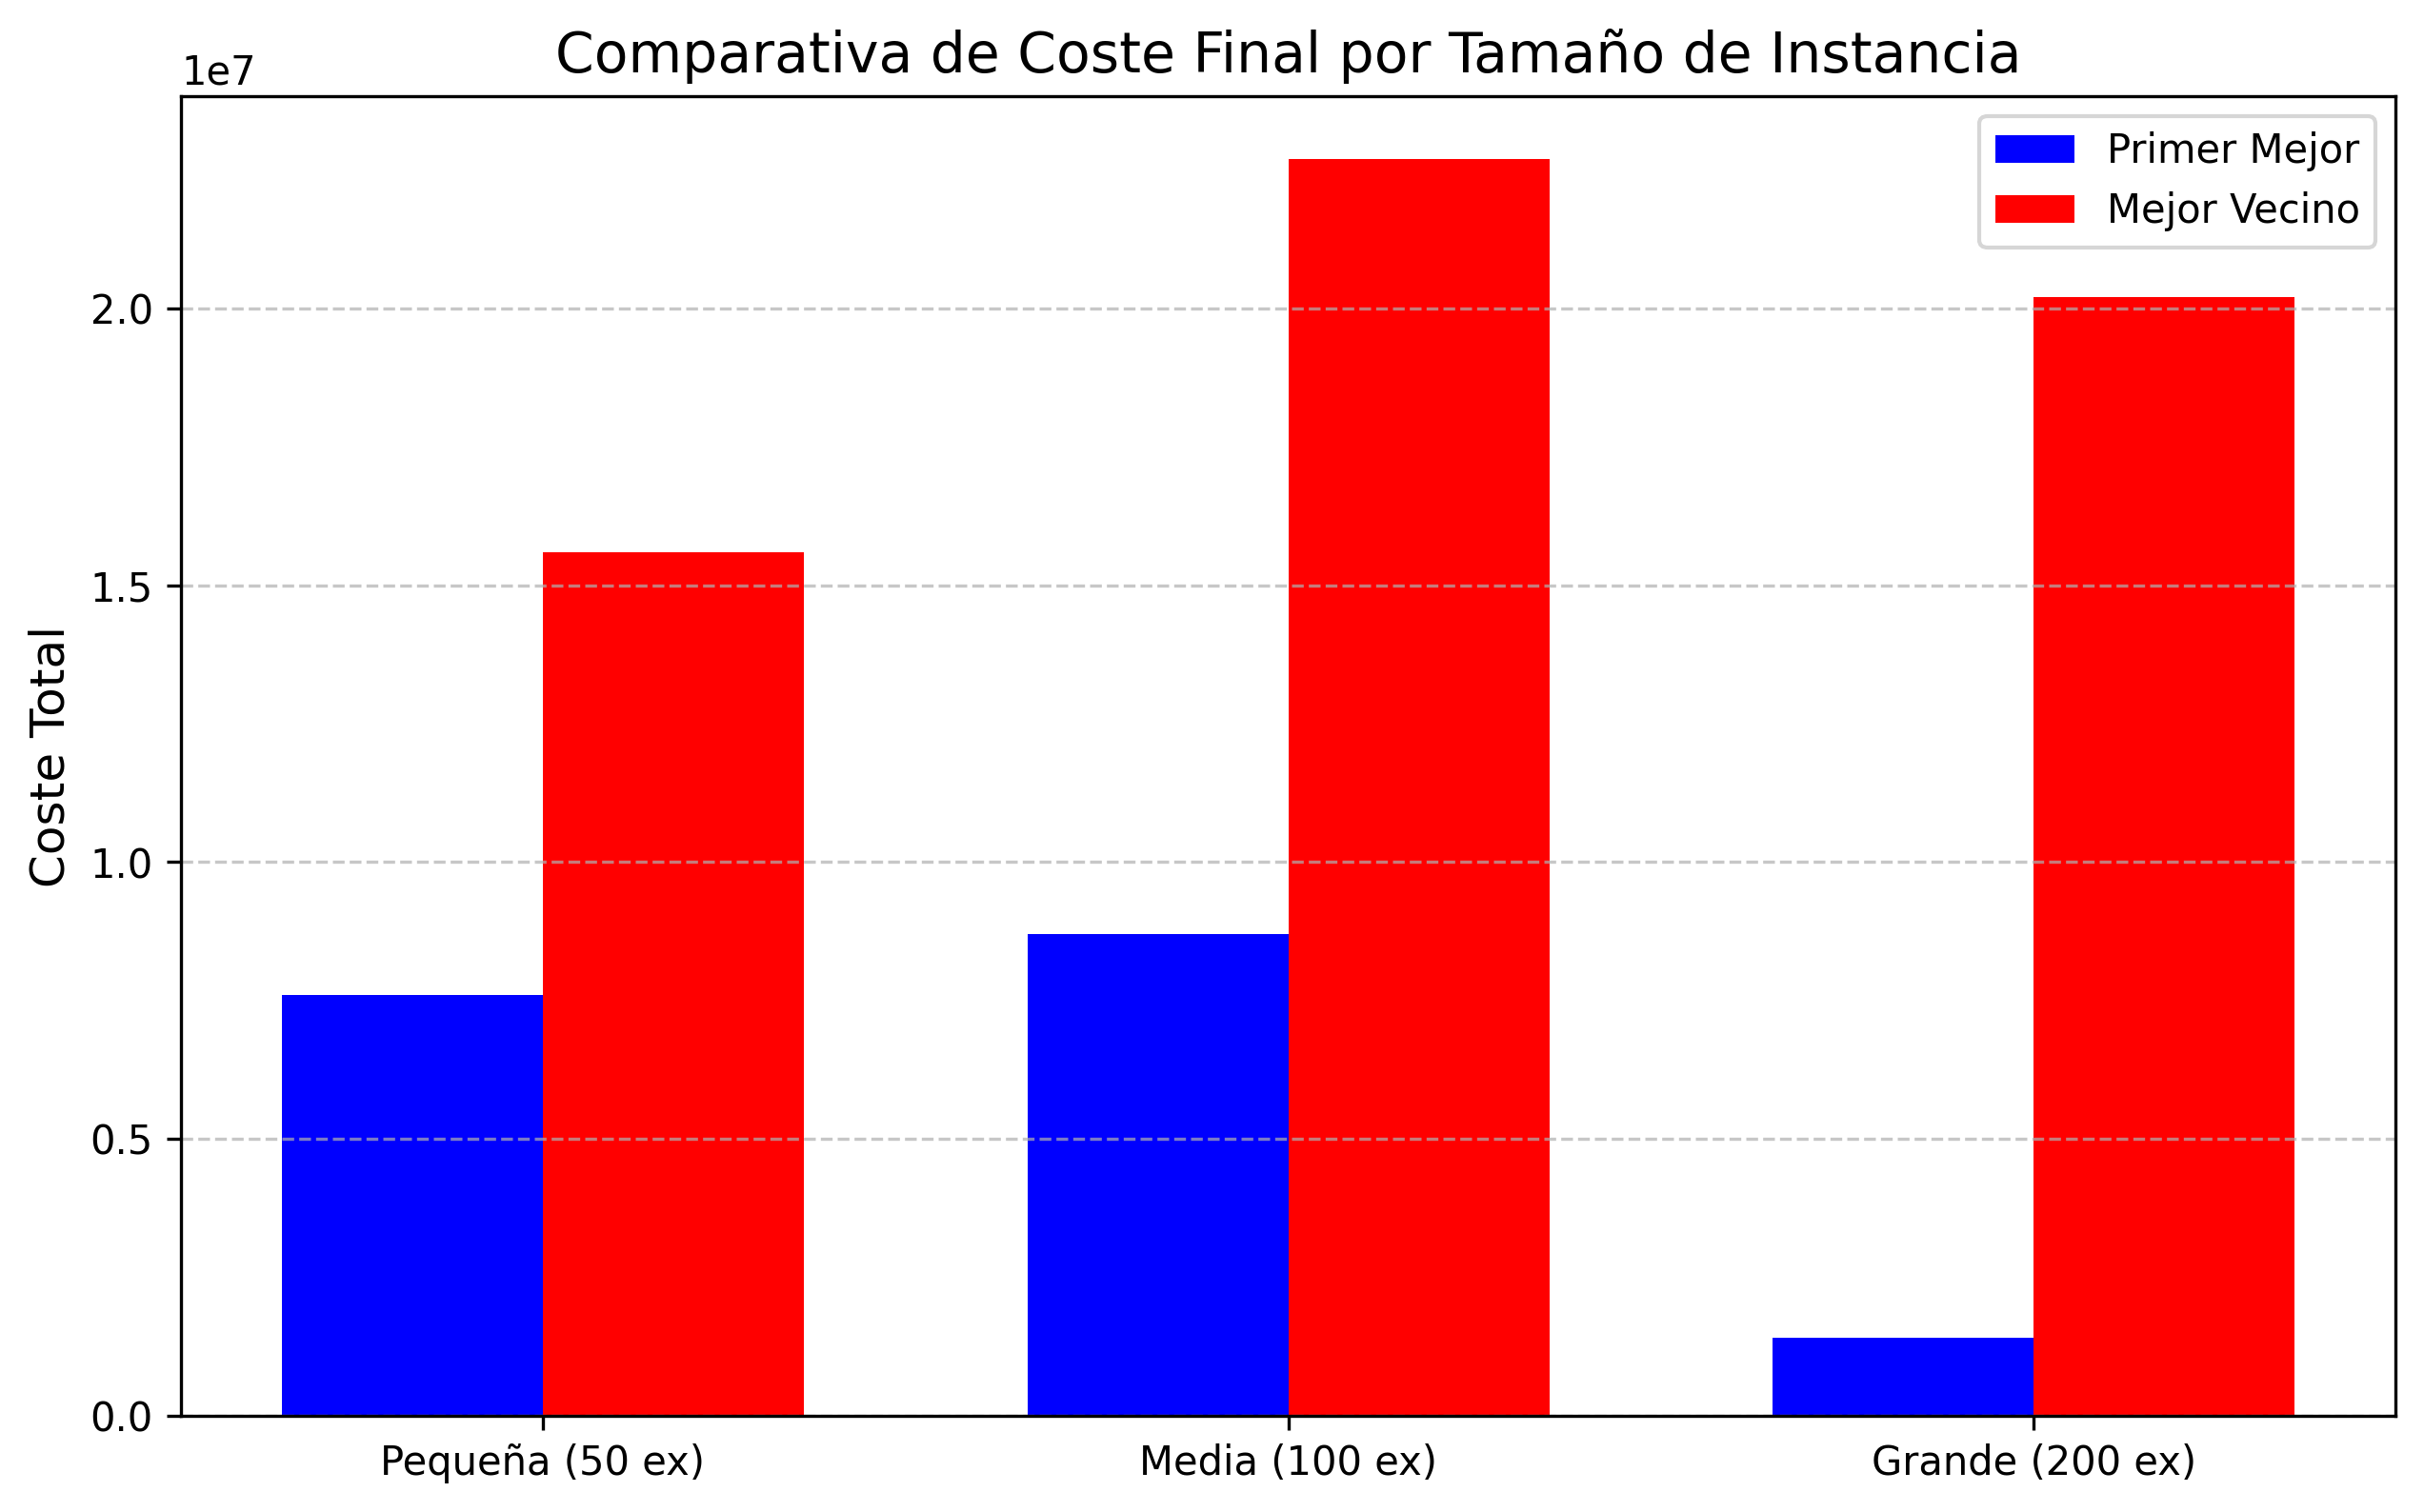
\includegraphics[width=0.7\textwidth]{graficas/comparativa_costes.png} 
    \caption{Evolución del coste de restricciones duras según el algoritmo utilizado.}
\end{figure}

\subsection{Escalabilidad: Comparativa según el tamaño de la instancia}
Siguiendo las recomendaciones del enunciado de la práctica, he querido comprobar cómo se comportan mis algoritmos y mi estructura de datos a medida que el problema crece. Para ello, he generado tres escenarios distintos modificando los parámetros del generador de instancias (\texttt{n\_exams}, \texttt{n\_students}, \texttt{n\_rooms} y \texttt{n\_slots}), manteniendo siempre la misma semilla (\texttt{seed=42}) para aislar la aleatoriedad.

Los tres escenarios planteados son:
\begin{itemize}
    \item \textbf{Instancia Pequeña:} 50 exámenes, 1000 estudiantes, 5 aulas y 25 slots.
    \item \textbf{Instancia Media (Base):} 100 exámenes, 2000 estudiantes, 10 aulas y 40 slots.
    \item \textbf{Instancia Grande:} 200 exámenes, 4000 estudiantes, 20 aulas y 100 slots.
\end{itemize}

A continuación, presento una tabla comparando cómo ha escalado la estrategia del Primer Mejor frente a la del Mejor Vecino en términos de Coste Total y Tiempo de Ejecución en estos tres escenarios:

\begin{table}[H]
\centering
\resizebox{\textwidth}{!}{
\begin{tabular}{lrrrr}
\toprule
\textbf{Tamaño de Instancia} & \textbf{Coste (Primer Mejor)} & \textbf{Coste (Mejor Vecino)} & \textbf{Tiempo PM} & \textbf{Tiempo MV} \\
\midrule
Pequeña (50 Exámenes) & 7,603,153.08 & 15,603,290.56 & 9.35 s & 23.33 s \\
Media (100 Exámenes) & 8,704,058.30 & 22,704,264.95 & 45.29 s & 48.84 s \\
Grande (200 Exámenes) & 1,402,980.58 & 20,203,681.20 & 99.14 s & 96.19 s \\
\bottomrule
\end{tabular}
}
\caption{Resultados de escalabilidad según el tamaño de instancia.}
\end{table}

Como se puede observar en los datos empíricos, la combinatoria del problema afecta fuertemente a los resultados y a los tiempos computacionales, pero nos permite observar un comportamiento muy interesante de ambas metaheurísticas.

Por un lado, con un límite fijo de 5000 evaluaciones, al algoritmo del Mejor Vecino le resulta prácticamente imposible acercarse a cero incumplimientos de las restricciones duras a medida que el problema crece. Analizar una muestra de 500 vecinos por iteración le resulta totalmente ineficiente cuando el espacio de búsqueda es tan inmenso, limitando al algoritmo a realizar apenas 10 iteraciones (mejoras reales) en los tres escenarios ya que al explorar cada vecindario al completo y tener solo 5000 evaluaciones, solo puede conseguir 10 iteraciones / mejoras (5000 evaluaciones / 500 límite por iteracion = 10 iteraciones).

Sin embargo, esta prueba confirma y enfatiza la conclusión extraída en el escenario base: la estrategia del Primer Mejor escala de una forma excepcionalmente buena. Gracias a su agresividad descendente, logra penetrar mucho más rápido en el espacio de búsqueda y explorar nuevos escenarios. Resulta especialmente impactante el caso de la instancia Grande (200 exámenes): mientras que el Mejor Vecino se quedó estancado en un coste de más de 20 millones (con 202 restricciones duras incumplidas), el Primer Mejor logró realizar 256 iteraciones de mejora continua, reduciendo el coste a tan solo 1.4 millones y dejando únicamente 14 conflictos en las restricciones duras.

Aunque en las instancias grandes el tiempo de ejecución lógicamente aumenta (rozando los 100 segundos), la diferencia de calidad en la solución generada demuestra que priorizar la velocidad de descenso sobre la exhaustividad local es la decisión de diseño más acertada para este tipo de problemas, siempre teniendo en cuenta que cada situación o problema al que me pueda enfrentar es un mundo y habría que estudiarlo en profundidad.

\begin{figure}[H]
    \centering
    \begin{minipage}{0.48\textwidth}
        \centering
        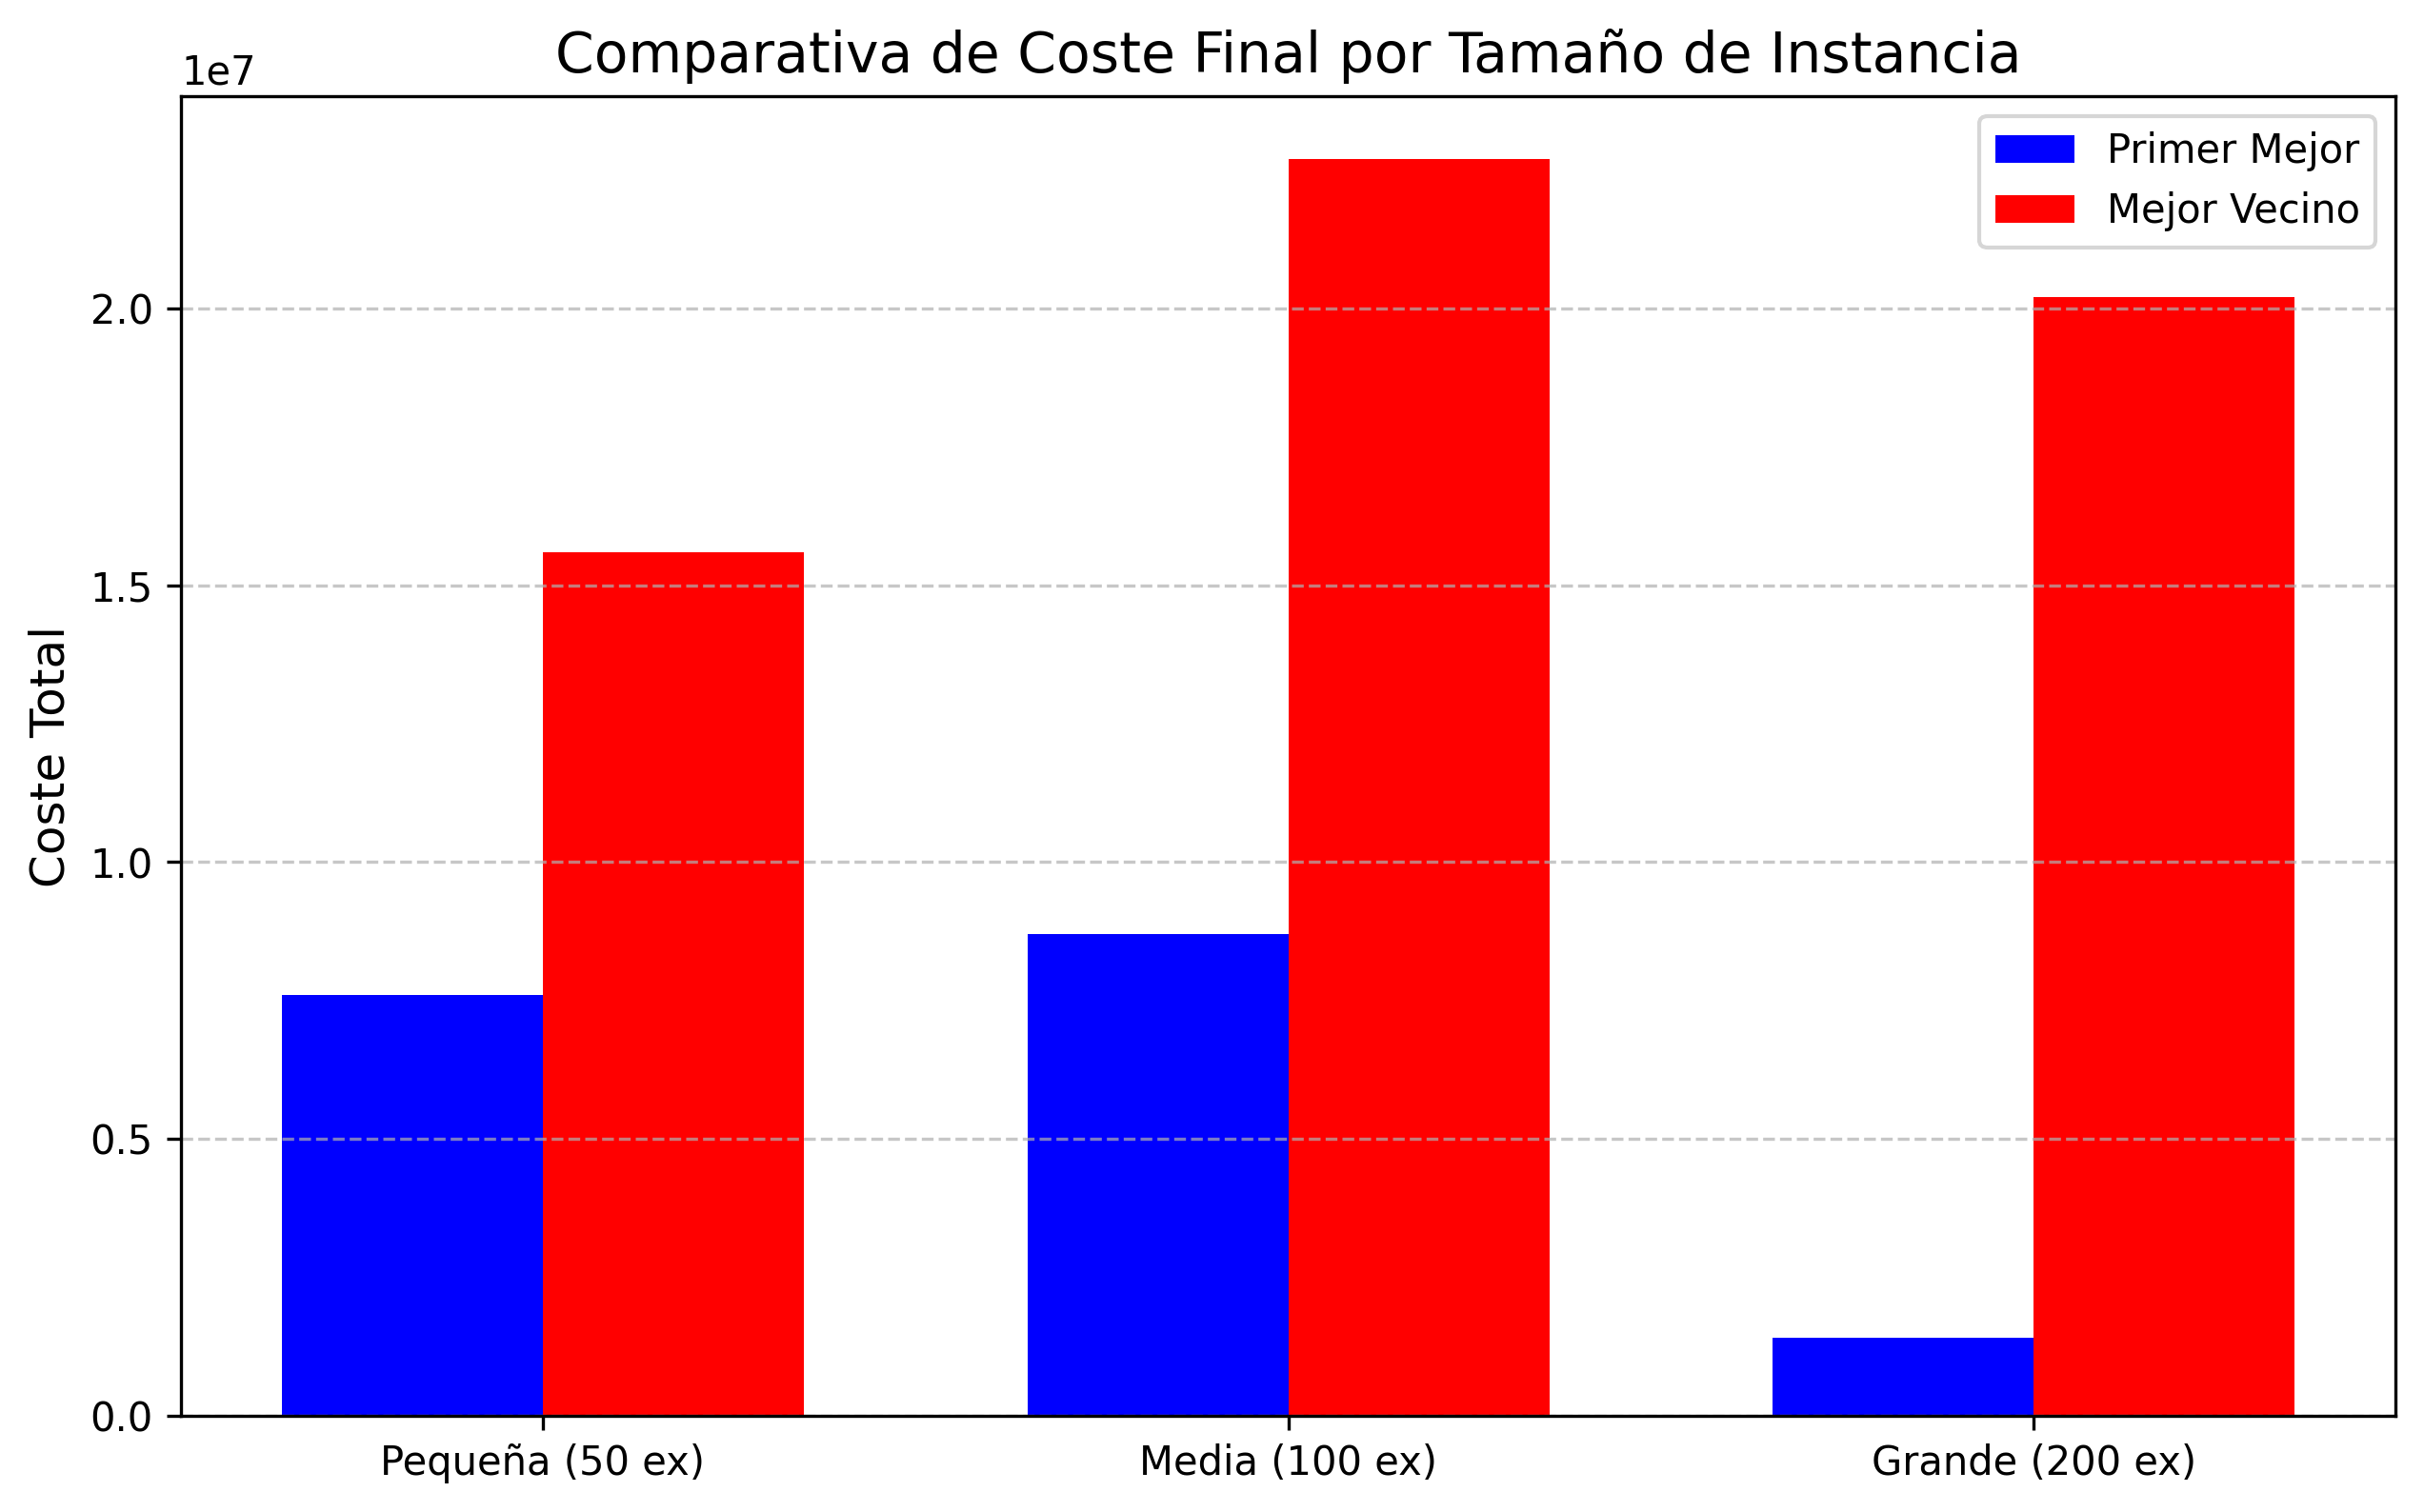
\includegraphics[width=\linewidth]{graficas/comparativa_costes.png}
        \caption{Comparativa de Costes.}
    \end{minipage}\hfill
    \begin{minipage}{0.48\textwidth}
        \centering
        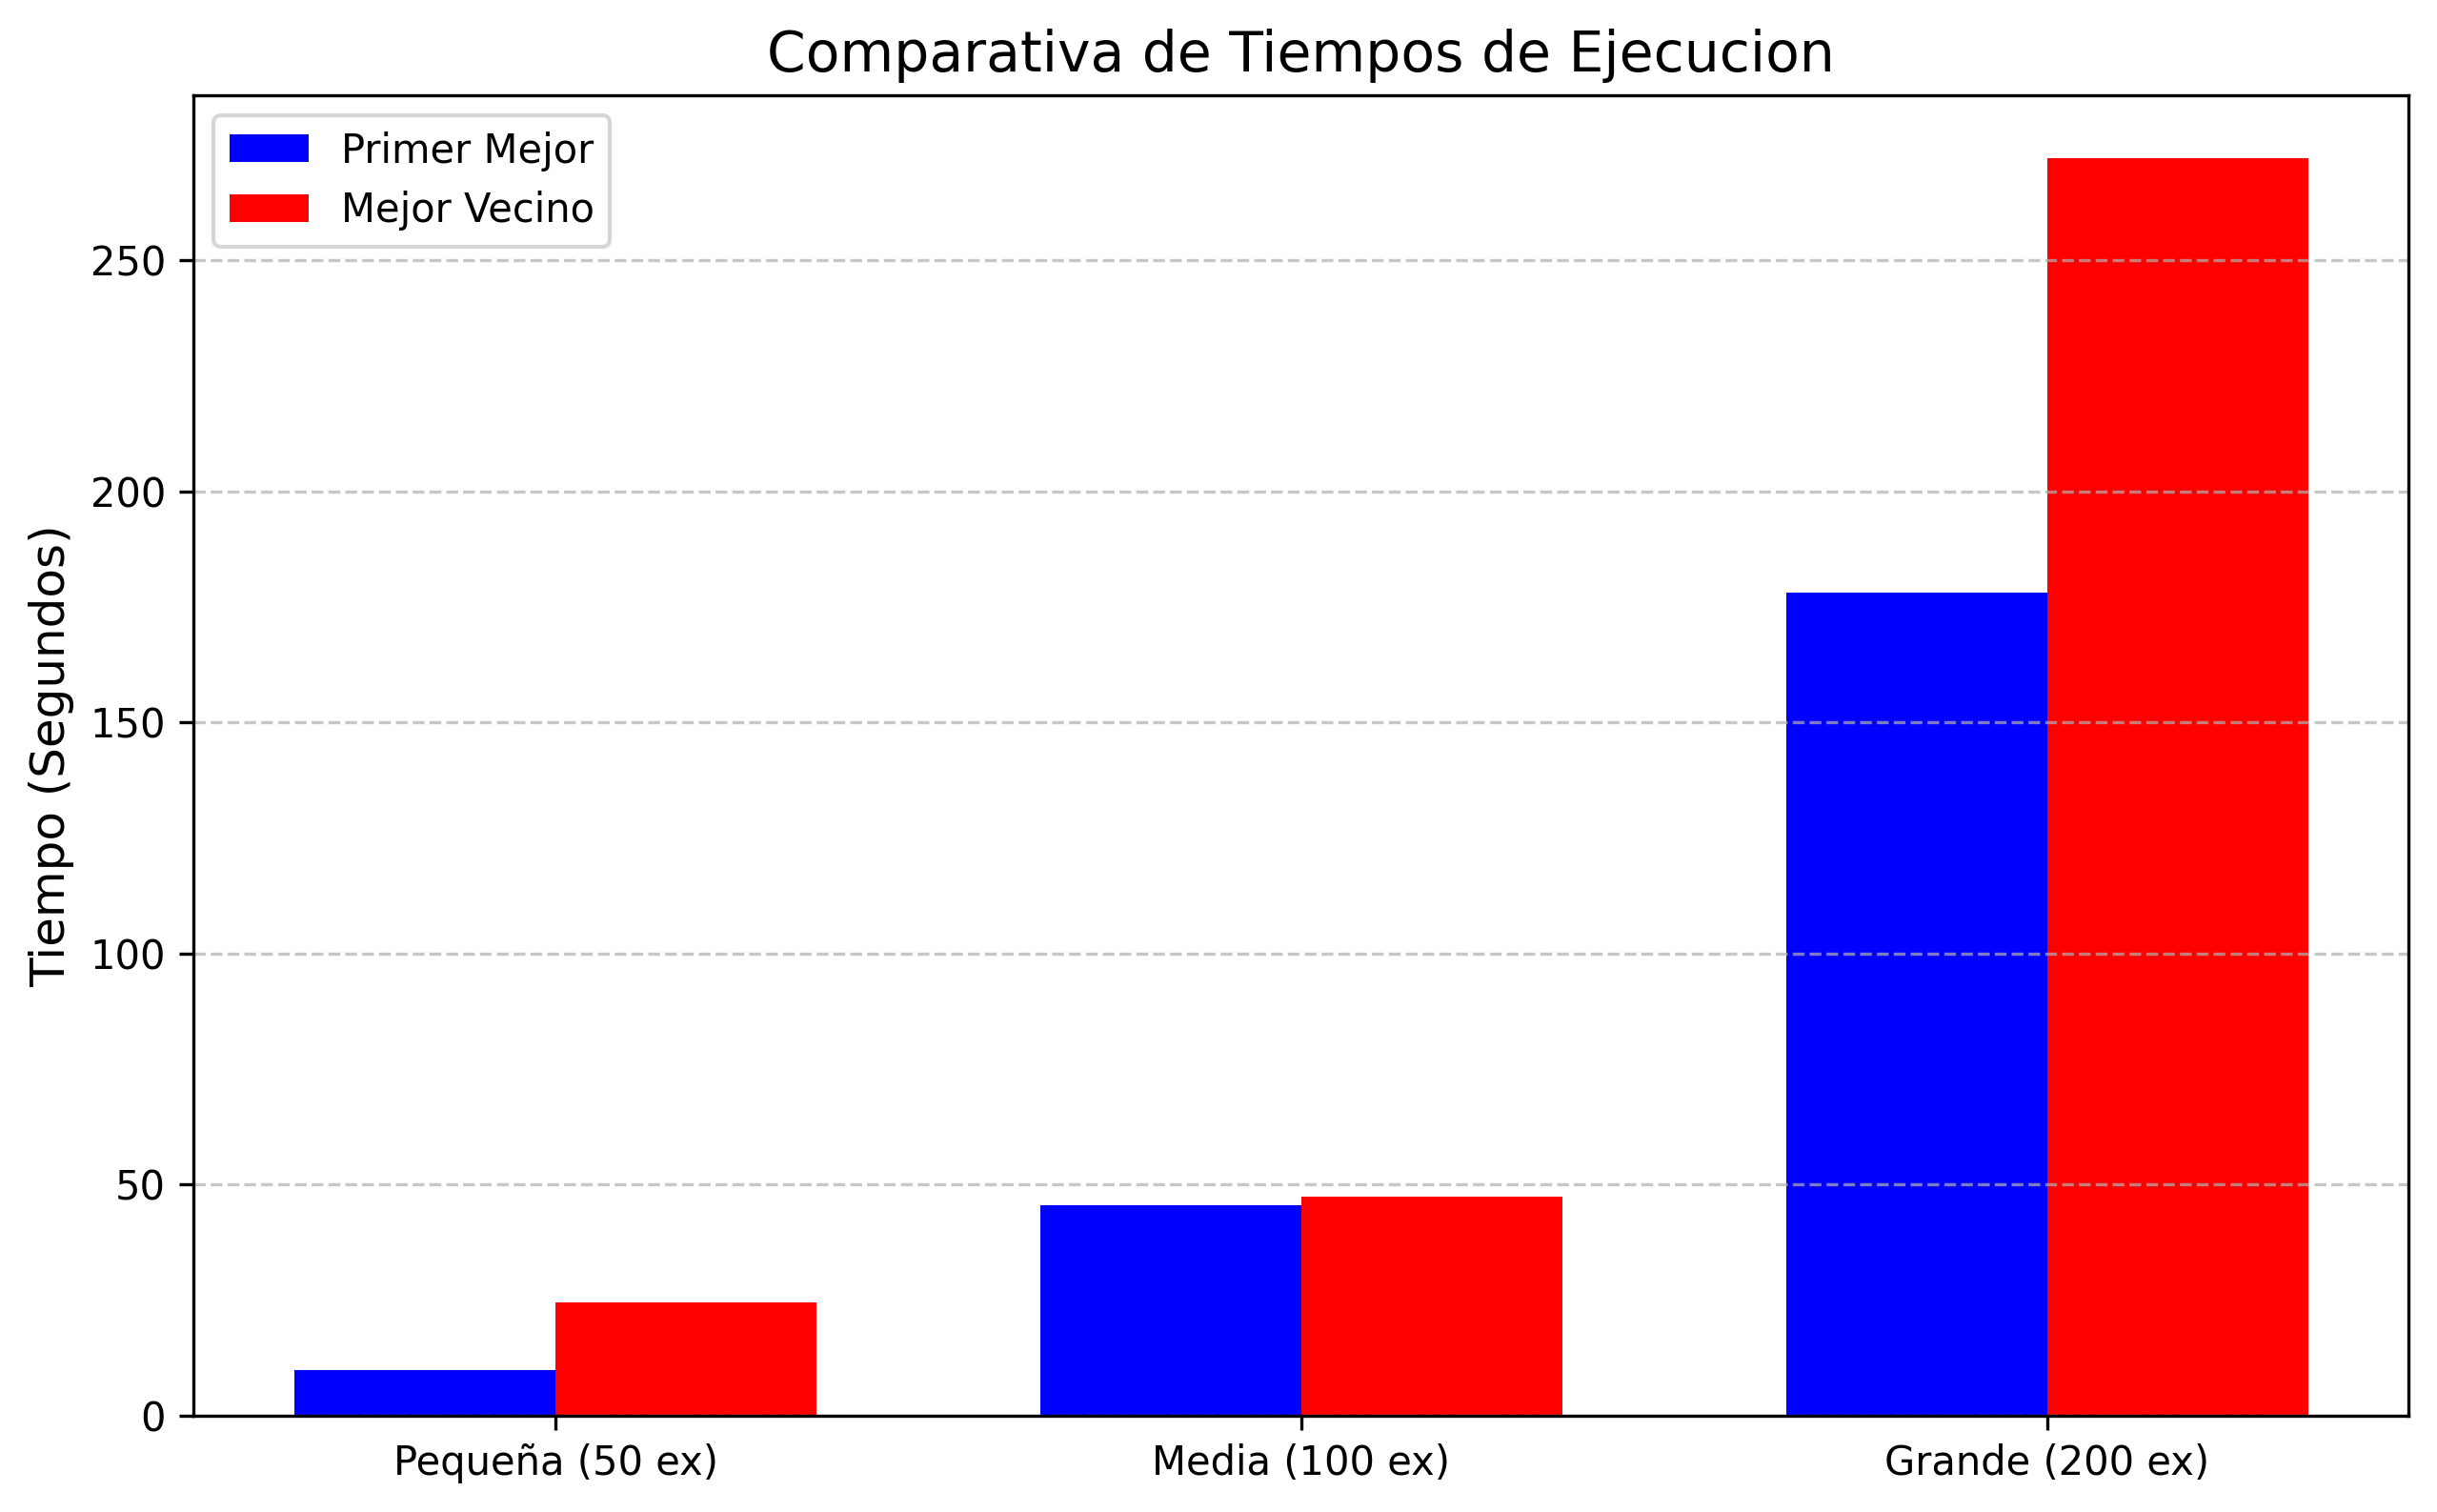
\includegraphics[width=\linewidth]{graficas/comparativa_tiempos.png}
        \caption{Comparativa de Tiempos.}
    \end{minipage}
\end{figure}

Para ilustrar de forma más visual la brecha de rendimiento entre ambas estrategias a medida que el problema crece, se presentan las siguientes gráficas comparativas. En ellas se aprecia claramente cómo el Primer Mejor (azul) mantiene un crecimiento controlado tanto en la calidad de la solución como en el tiempo invertido, mientras que el Mejor Vecino (rojo) sufre una degradación muy severa en su coste final al enfrentarse a espacios de búsqueda más amplios.

\section{Análisis de resultados}
Tomando como referencia los datos obtenidos en la ejecución con la Instancia Media (100 exámenes), la comparativa de algoritmos de búsqueda local revela un comportamiento bastante interesante que demuestra la teoría de las metaheurísticas en la práctica.

En primer lugar, se aprecia que la solución inicial (aleatoria) es bastante mala y altamente costosa, actuando únicamente como un comodín a partir del cuál empezar a encontrar mejoras rápido con los algoritmos.

Lo verdaderamente destacable es que la estrategia de Primer Mejor ha dado un resultado más eficiente con una diferencia abismal con respecto al de la estrategia del Mejor Vecino, obteniendo un coste muchísimo menor (8.7 millones frente a 22.7 millones) y reduciendo los incumplimientos a casi un tercio, invirtiendo además un poco menos de tiempo.

\begin{figure}[H]
    \centering
    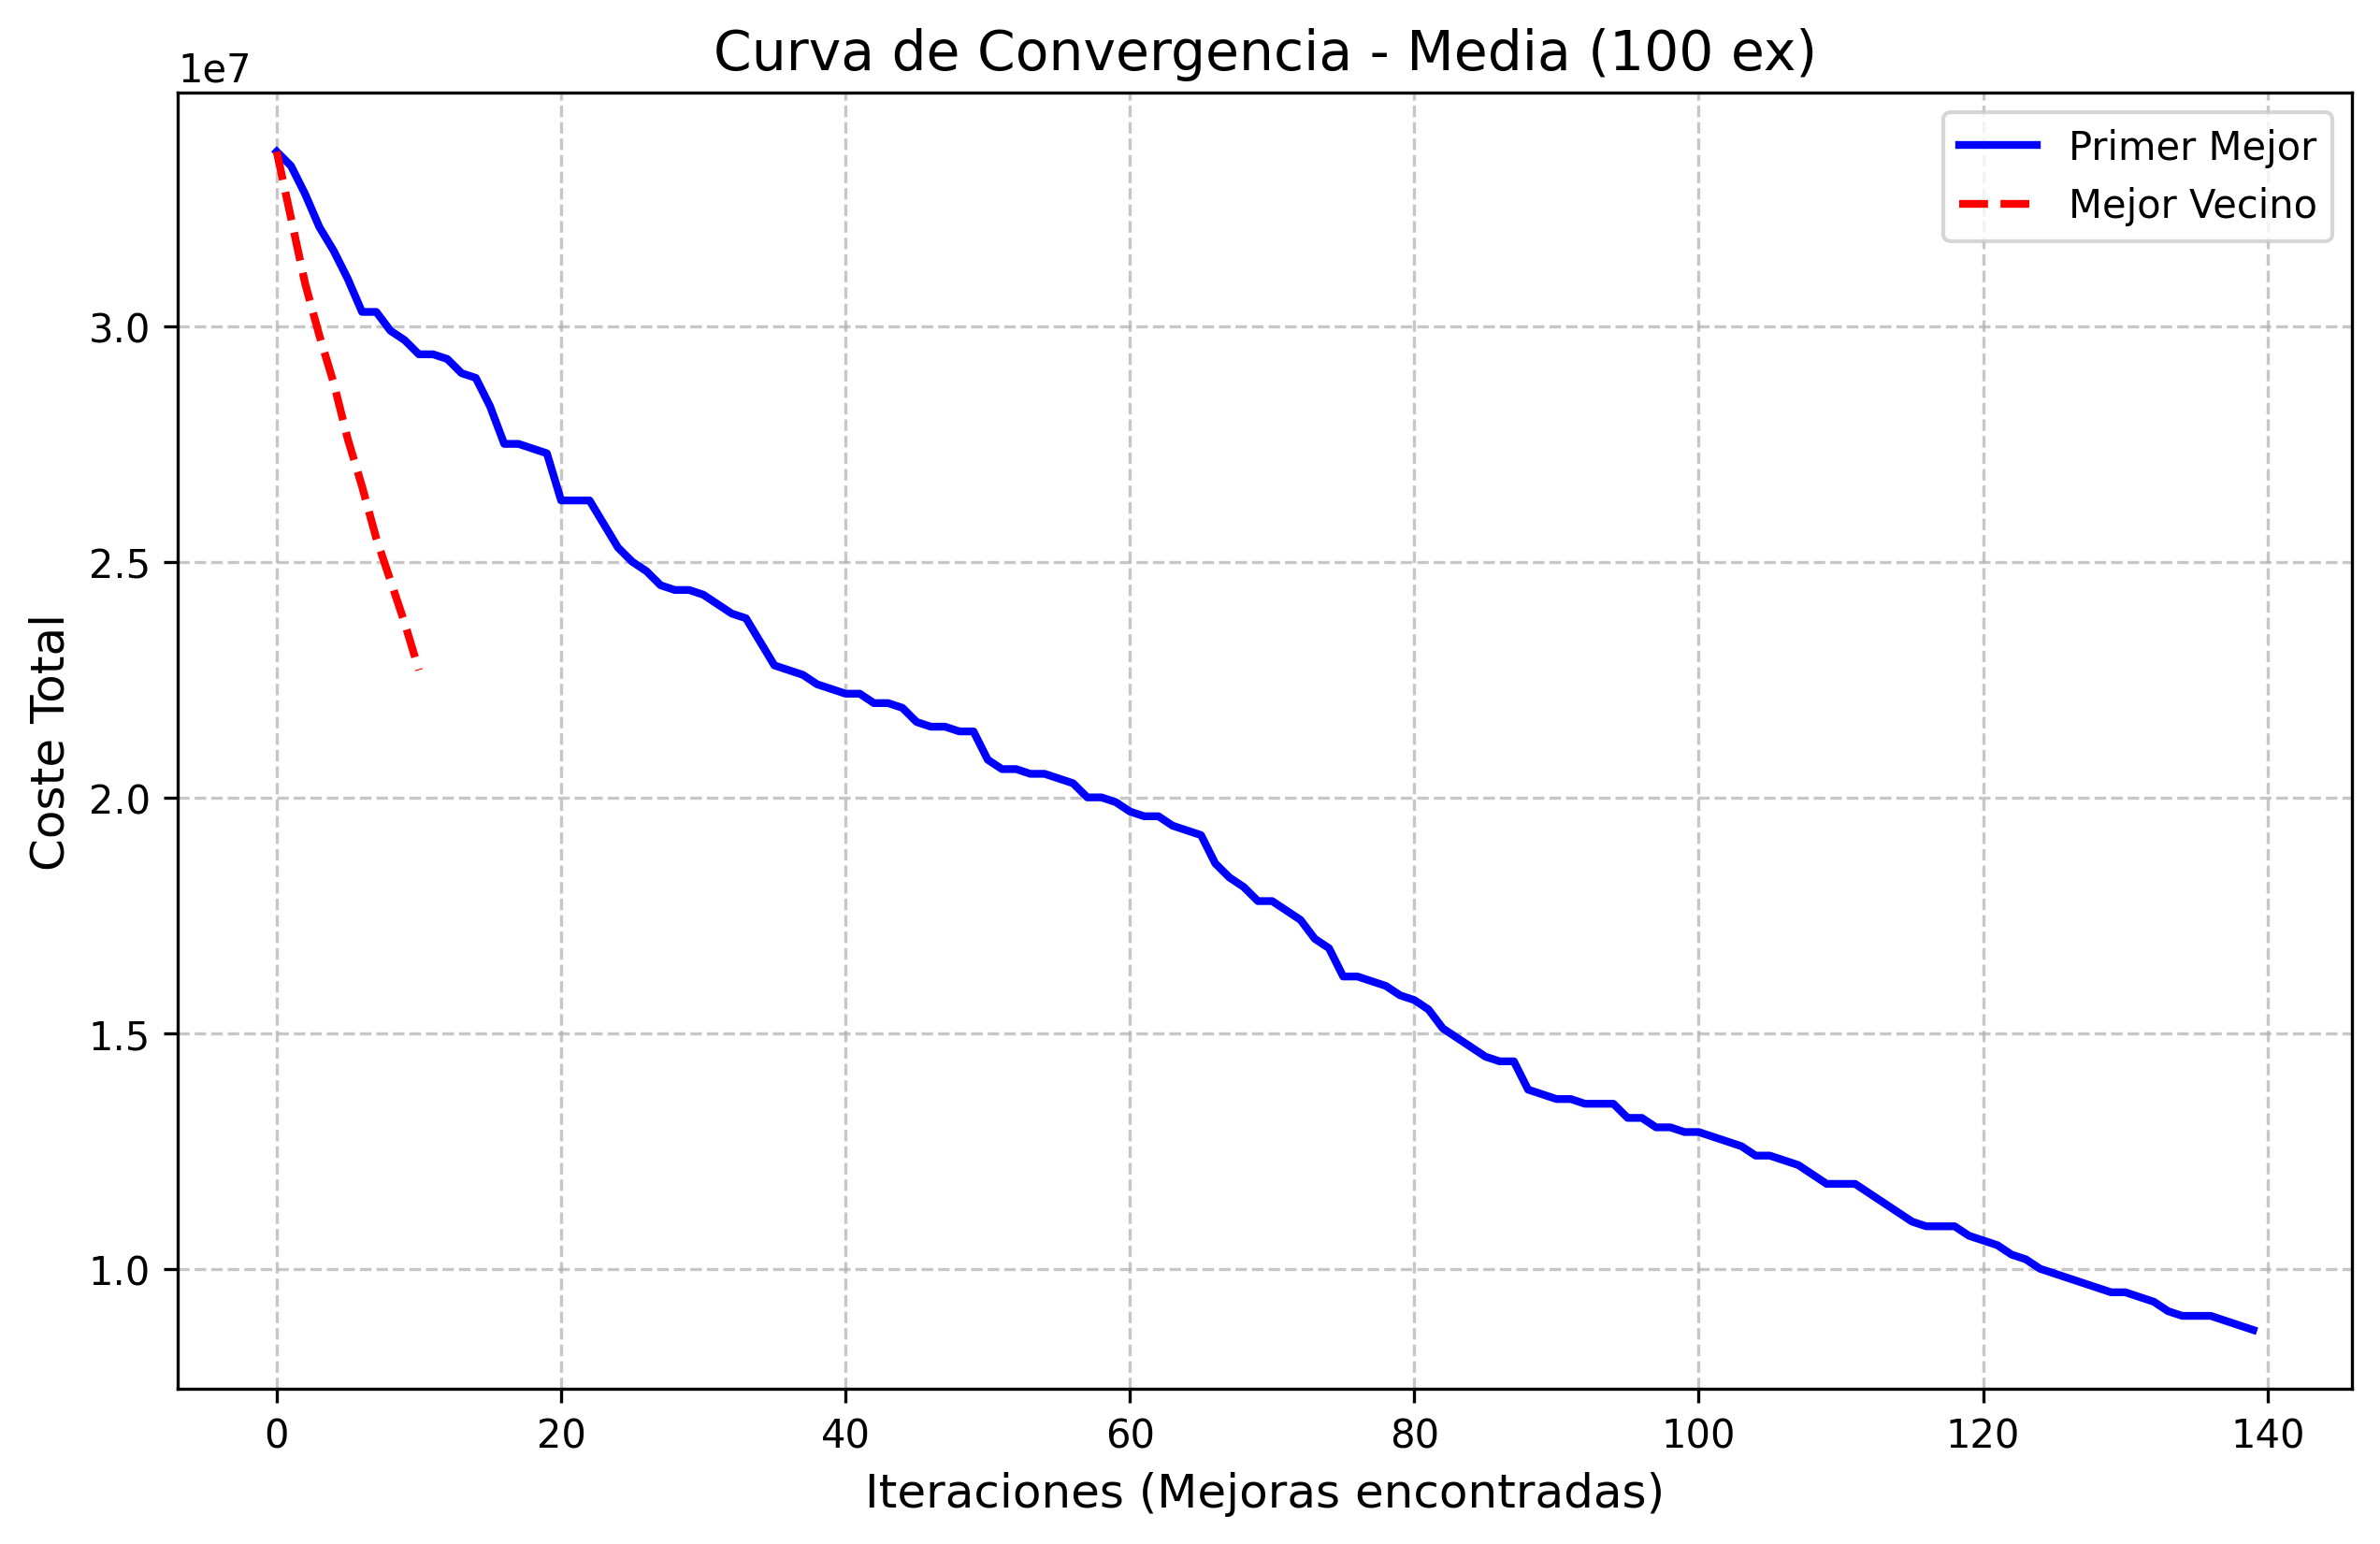
\includegraphics[width=0.8\textwidth]{graficas/convergencia_Media_100_ex.png}
    \caption{Curva de convergencia en la Instancia Media.}
\end{figure}

Este suceso tiene una justificación técnica muy clara analizando los datos obtenidos: Al haber configurado el "Mejor Vecino" para que genere y evalúe 500 vecinos en cada iteración, el algoritmo consume sus 5000 evaluaciones permitidas en apenas 10 iteraciones (500 x 10 = 5000). Es decir, en todo el proceso de búsqueda, la solución solo ha dado 10 pasos en el espacio de búsqueda. Ha sido muy profundo evaluando su entorno y cada vecindario, pero se ha movido muy poco, por lo que realmente el margen de mejora se ve muy condicionado por eso mismo.

Por el contrario, la estrategia de "Primer Mejor" es muy agresiva y rápida. Acepta la primera mejora que encuentra sin analizar todo el vecindario. Como podemos ver en los resultados, con 4702 evaluaciones ha sido capaz de hacer 139 iteraciones (evaluaciones con mejora). Es decir, el Primer Mejor ha descendido por el gradiente de la función objetivo 139 veces, alejándose muchísimo más de la mala solución inicial y esquivando mejor los óptimos locales, mientras que el Mejor Vecino se quedó analizando y solo dio 10 iteraciones, por lo que el “campo” explorado es mucho más reducido y por ende el resultado que devuelve es más pobre.

\subsection{Análisis visual de la convergencia por tamaño de instancia}
Para ilustrar de forma gráfica las conclusiones que he extraido sobre la escalabilidad, resulta fundamental observar no solo el coste final obtenido, sino el "camino" que ha recorrido cada metaheurística. Al graficar la evolución del coste frente al número de iteraciones (mejoras reales aplicadas), el comportamiento de ambos algoritmos queda totalmente al descubierto.

% AQUÍ ESTÁN LAS TRES GRÁFICAS JUNTAS (DOS ARRIBA Y UNA ABAJO)
\begin{figure}[H]
    \centering
    % Fila superior: Instancia Pequeña y Media
    \begin{minipage}{0.48\textwidth}
        \centering
        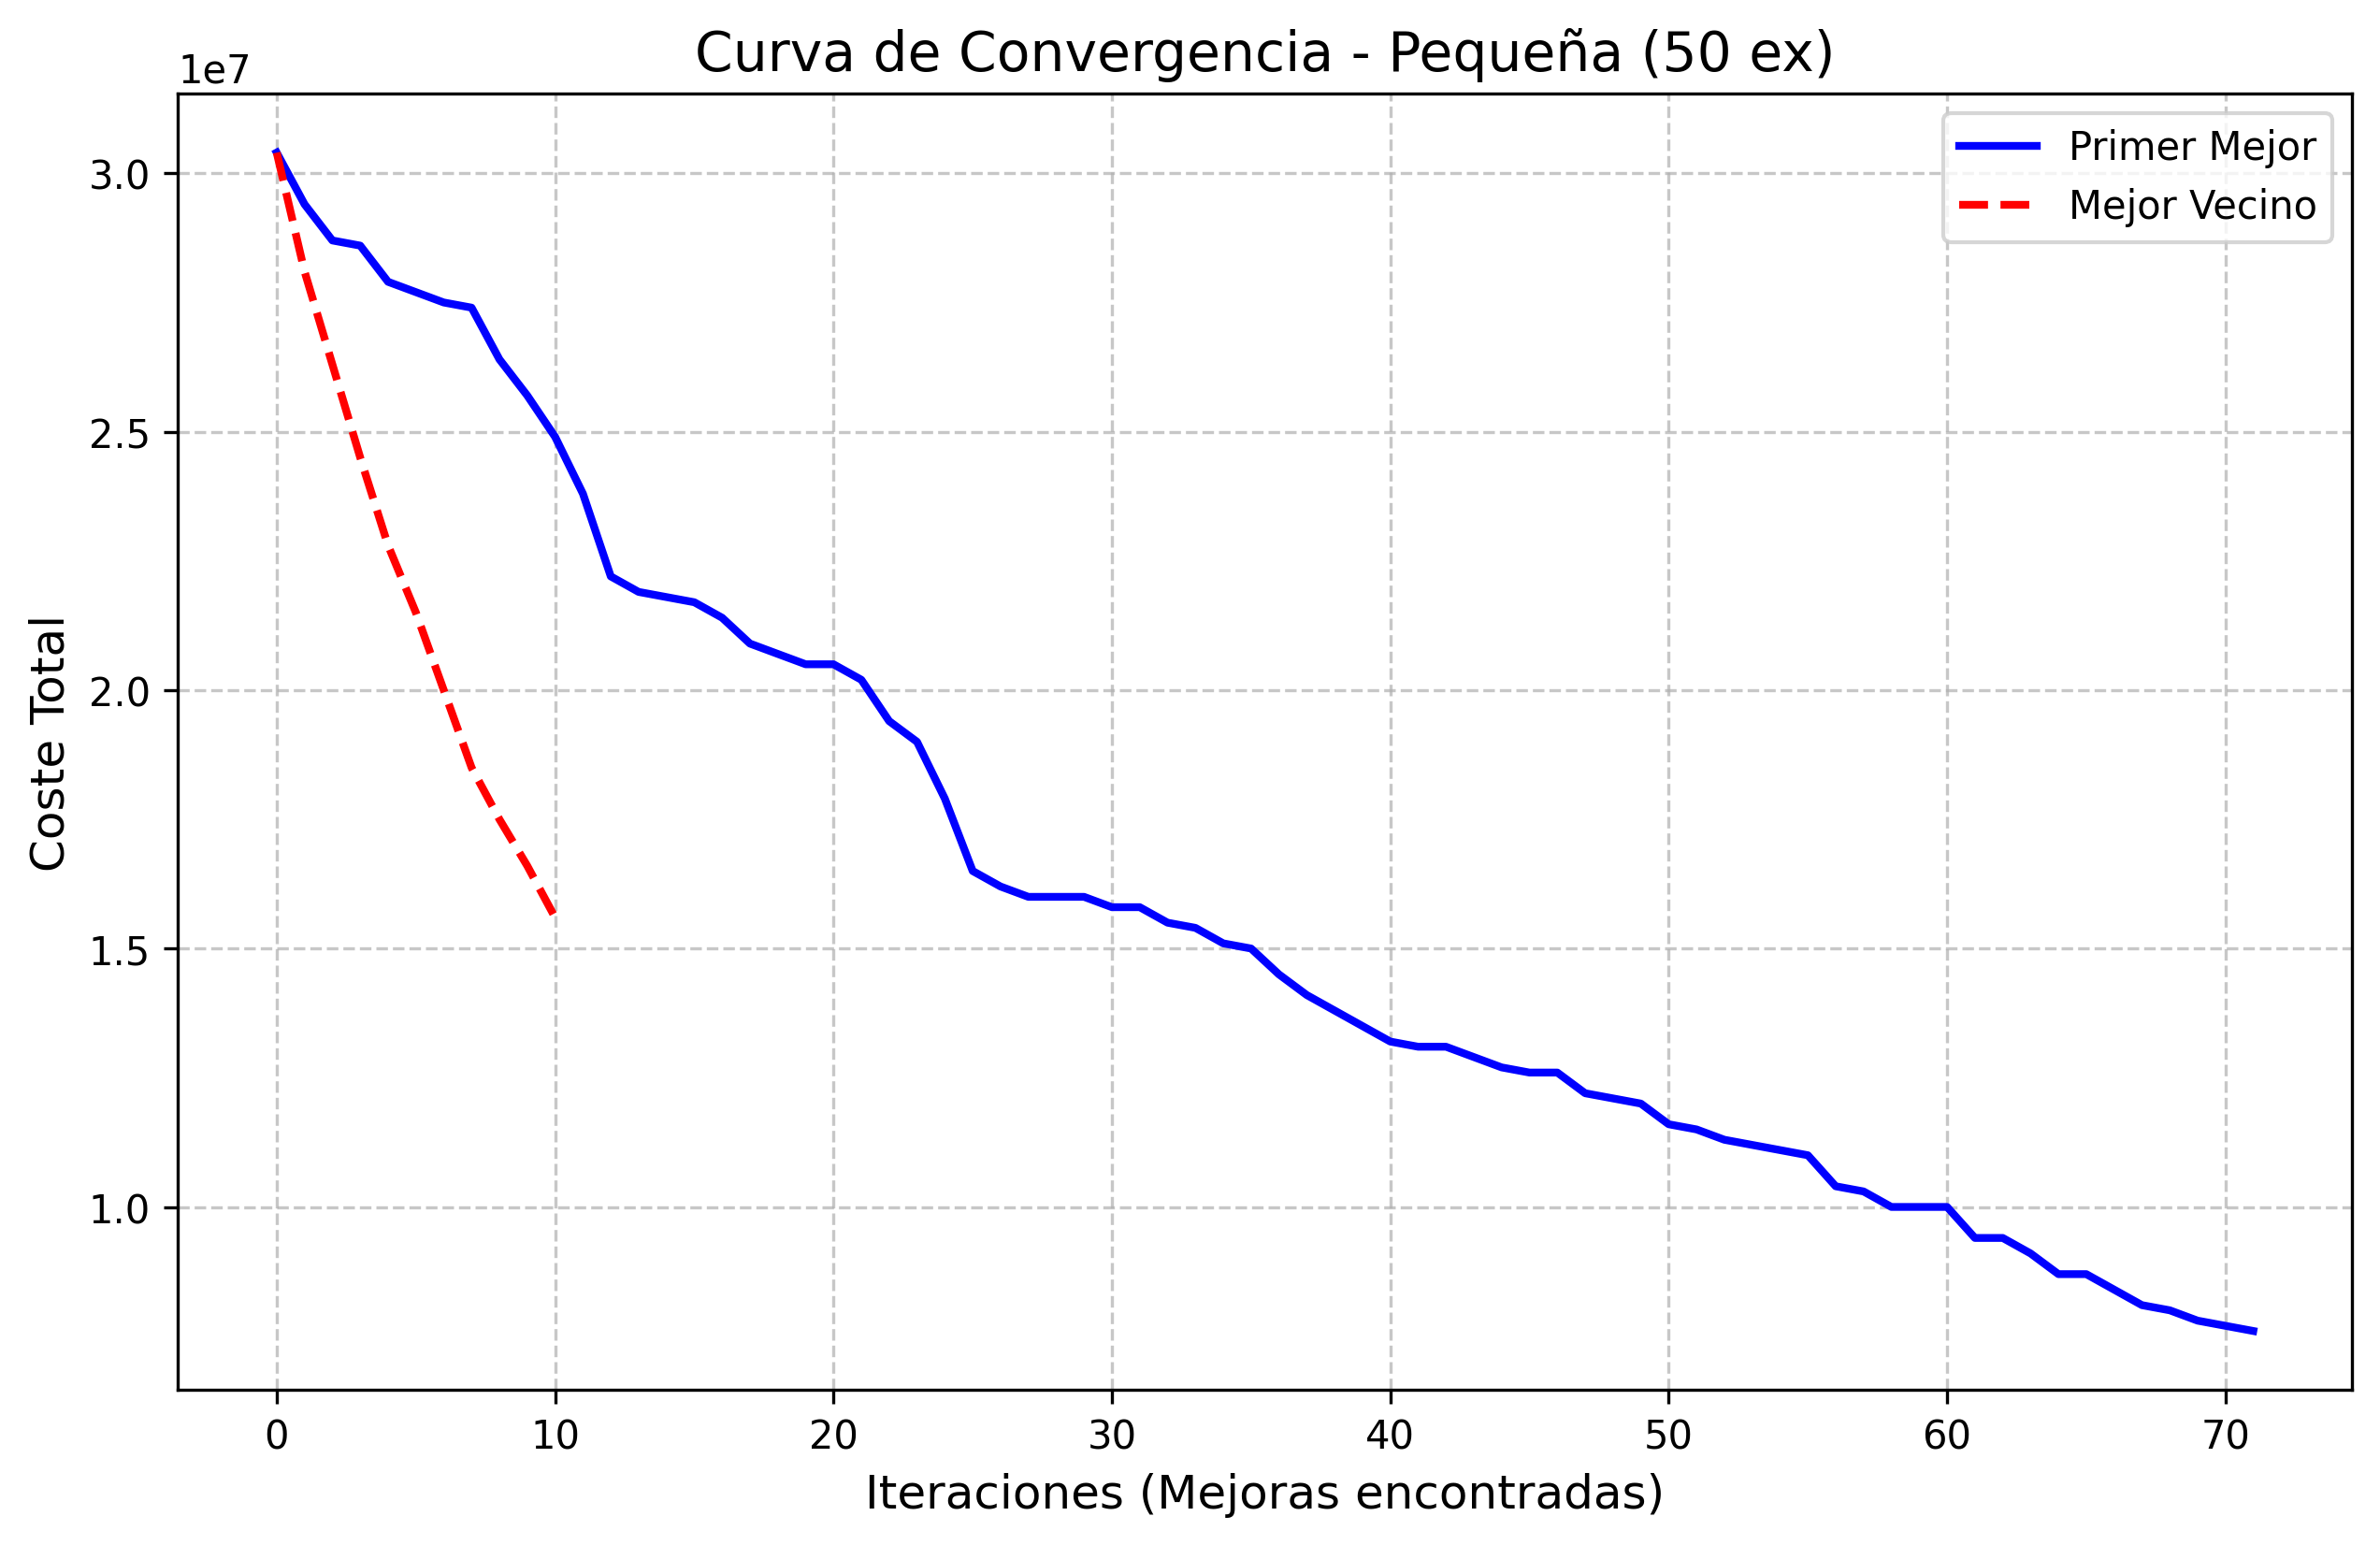
\includegraphics[width=\linewidth]{graficas/convergencia_Pequeña_50_ex.png}
        \caption{Convergencia: Pequeña.}
    \end{minipage}\hfill
    \begin{minipage}{0.48\textwidth}
        \centering
        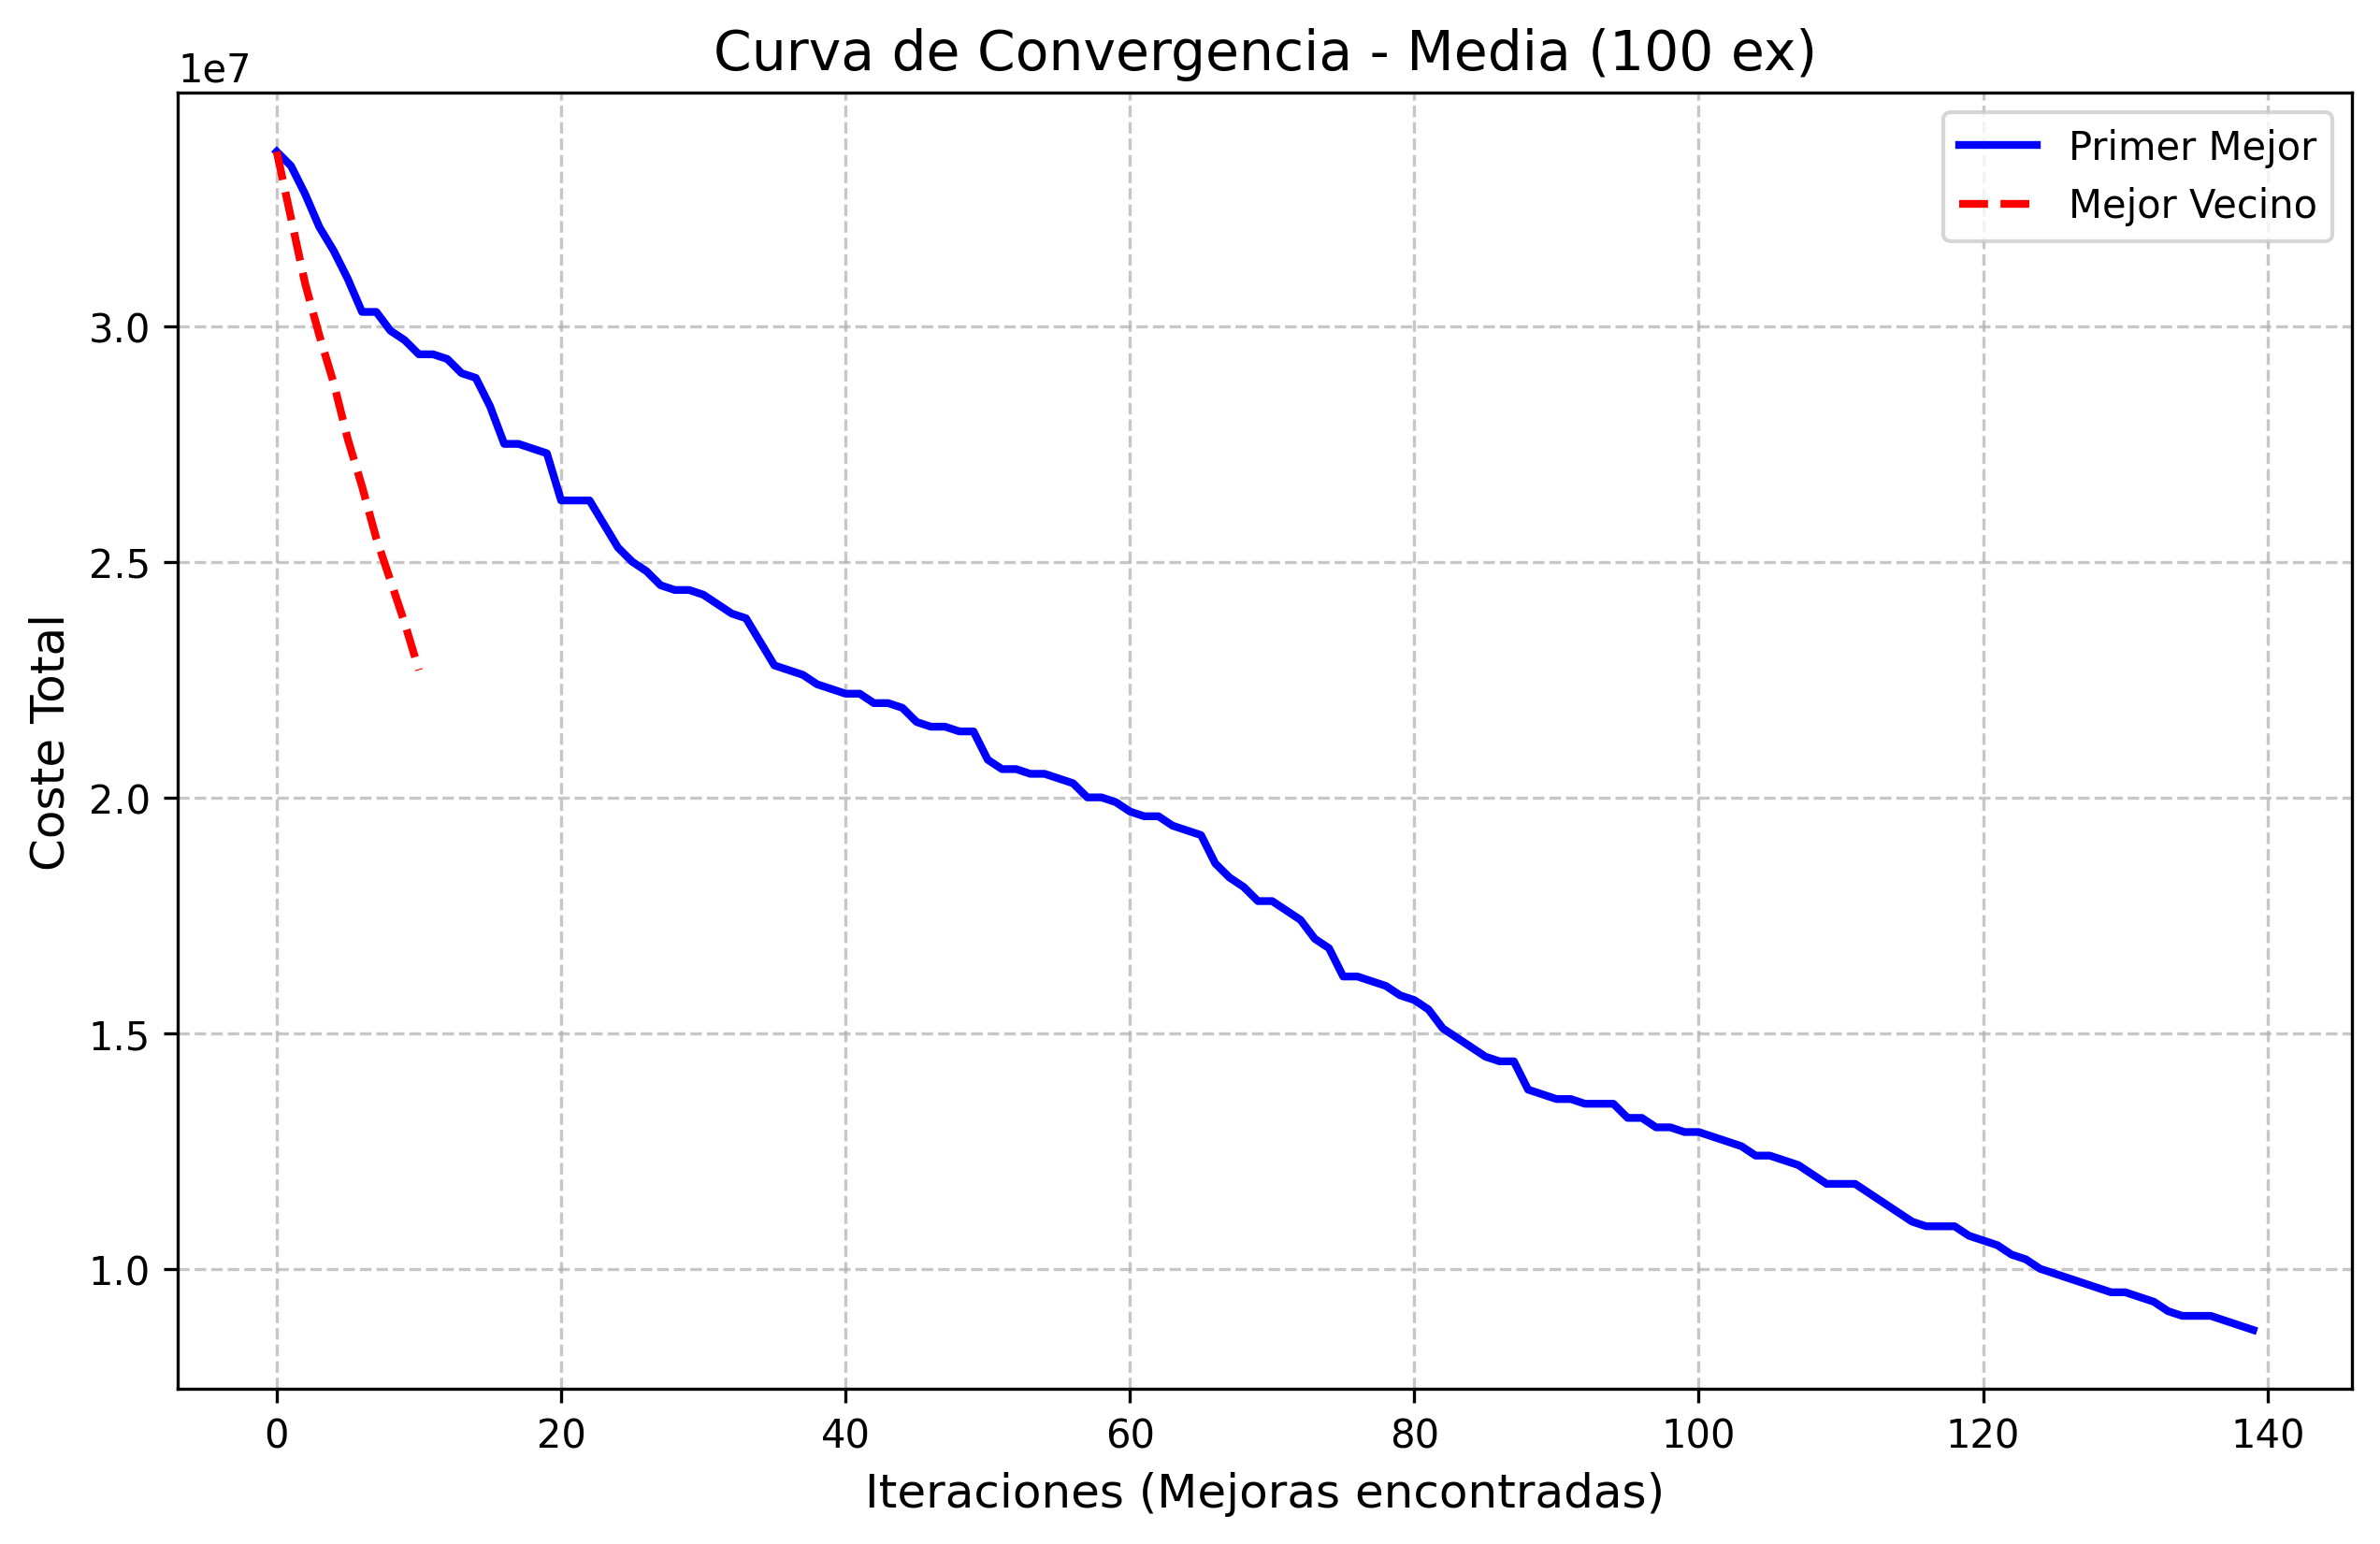
\includegraphics[width=\linewidth]{graficas/convergencia_Media_100_ex.png}
        \caption{Convergencia: Media.}
    \end{minipage}
    
    \vspace{0.5cm} % Un pequeño espacio para separar la fila de arriba con la de abajo
    
    % Fila inferior: Instancia Grande (centrada)
    \begin{minipage}{0.48\textwidth}
        \centering
        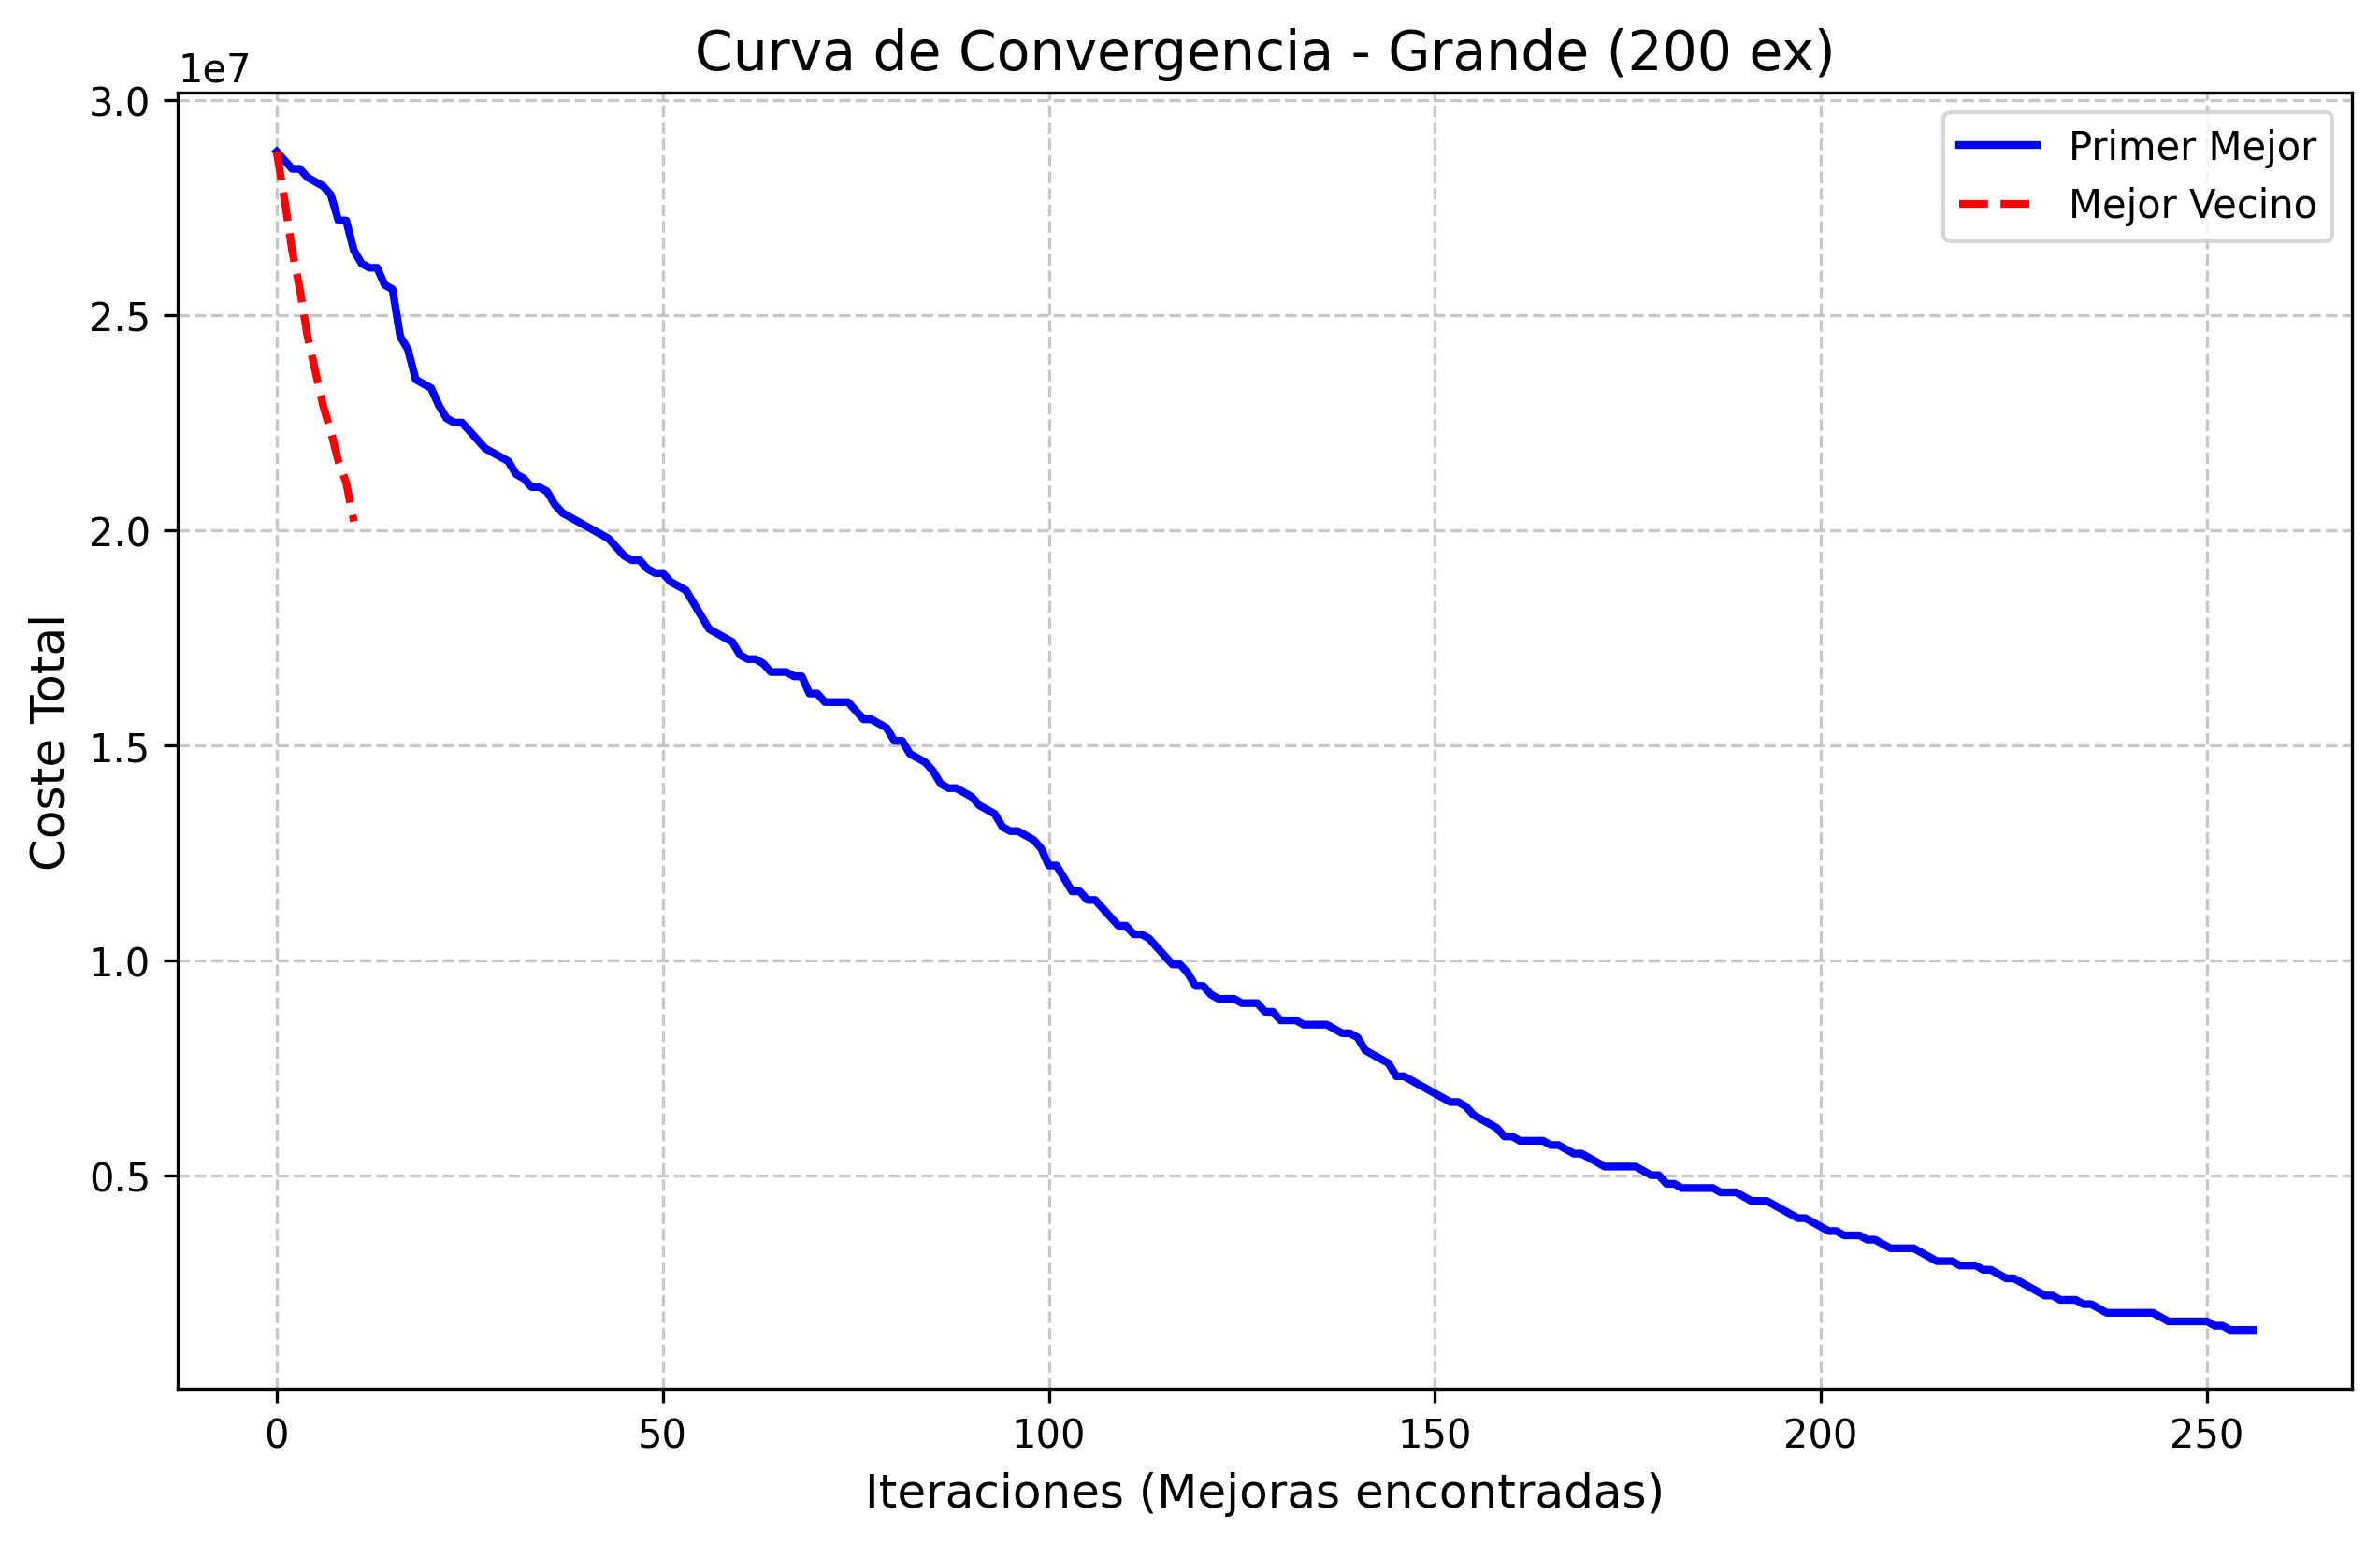
\includegraphics[width=\linewidth]{graficas/convergencia_Grande_200_ex.png}
        \caption{Convergencia: Grande.}
    \end{minipage}
\end{figure}

Analizando las curvas, el contraste es evidente y apoya nuestra teoría:
\begin{itemize}
    \item \textbf{En la instancia Pequeña (50 exámenes):} Ambos algoritmos logran descender y dibujar una curva, ya que el espacio de búsqueda es lo suficientemente abarcable como para que el Mejor Vecino pueda dar varios pasos (iteraciones) antes de agotar sus 5000 evaluaciones.
    \item \textbf{En las instancias Media y Grande:} La gráfica revela el colapso exploratorio del Mejor Vecino. Su "curva" se convierte prácticamente en una línea plana y cortísima que se interrumpe abruptamente en la iteración 10. Al tener vecindarios tan gigantescos, gasta todo su presupuesto de evaluaciones mirando a su alrededor sin apenas avanzar.
    \item Por el contrario, la línea del \textbf{Primer Mejor} demuestra un descenso por gradiente continuo y agresivo en los tres escenarios. En la instancia Grande, se puede observar perfectamente cómo, mientras el Mejor Vecino se rinde casi al inicio, el Primer Mejor sigue cayendo en picado durante más de 250 iteraciones, logrando penetrar mucho más profundo en el espacio de soluciones factibles.
\end{itemize}

Esta comparativa visual confirma definitivamente que, dado el estricto límite de 5000 evaluaciones, una estrategia de explotación rápida (Primer Mejor) es infinitamente superior a una estrategia de exploración exhaustiva local (Mejor Vecino) a medida que el problema sufre explosión combinatoria.

\section{Conclusiones}
Tras la realización de esta práctica he logrado modelar con éxito un problema de combinatoria, transformando restricciones que se dan en la vida real en una función matemática penalizada de forma balanceada.

He comprobado que:
\begin{itemize}
    \item Permitir transitar por estados infactibles aplicando penalizaciones desproporcionadas (100,000 por restricciones duras) es una técnica robusta. Permite a la Búsqueda Local pasar por conflictos de horarios inválidos sin quedarse atascada inmediatamente.
    \item Con respecto a los dos algoritmos me he dado cuenta de que en espacios de búsqueda gigantescos, la rapidez de descenso importa más que la exhaustividad local en la mayoría de los casos. Evaluar el mejor de 500 vecinos es una pérdida de tiempo computacional cuando ese mismo tiempo te permite dar 15 pasos aleatorios pero ascendentes con la técnica del Primer Mejor.
    \item El diseño de las estructuras de datos, como los diccionarios precalculados, es tan importante como el propio algoritmo de IA para lograr que la ejecución termine en un tiempo razonable.
\end{itemize}

Esta práctica ha supuesto un punto de inflexión en mi comprensión de la parte teórica de la asignatura y las metaheurísticas en general. Pensaba que comprendía a la perfección la teoría, pero al enfrentarme a las decisiones de ingeniería que requiere un problema real y desarrollarlo funcionalmente hay cuestiones que no sabía que tendría que tener en cuenta: qué estructura de datos usar para no saturar la CPU, cómo equilibrar matemáticamente una penalización, y cómo definir un vecindario variado.

Lo más gratificante ha sido la fase de análisis de resultados. Al ver los datos finales, he podido entender exactamente por qué el algoritmo del Mejor Vecino estaba comportándose peor que el Primer Mejor, lo cuál al principio me hizo creer que estaba haciendo mal. Ver esa relación directa entre las evaluaciones desperdiciadas y el número de iteraciones (los 10 pasos del Mejor Vecino frente a los 139 del Primer Mejor) ha sido clave. Ahora entiendo que, en optimización algorítmica, la estrategia que suena más "inteligente" o meticulosa en papel no siempre es la más adecuada para el contexto en el que se da y los límites de computación del mundo real tienen un papel fundamental a la hora de tomar decisiones.

\end{document}